\documentclass[conference]{IEEEtran}

\usepackage{cite}
\usepackage{amsmath,amssymb,amsfonts}
\usepackage{algorithmic}
\usepackage{algorithm}
\usepackage{graphicx}
\usepackage{textcomp}
\usepackage{xcolor}
\usepackage{booktabs}
\usepackage{multirow}
\usepackage{array}
\usepackage{url}
\usepackage{microtype}
\setlength{\emergencystretch}{1em}

% TikZ and vector graphics packages
\usepackage{tikz}
\usetikzlibrary{shapes.geometric, arrows.meta, positioning, calc, fit, backgrounds}


% Graphicspath declaration
\graphicspath{{figures/}}

\def\BibTeX{{\rm B\kern-.05em{\sc i\kern-.025em b}\kern-.08em
    T\kern-.1667em\lower.7ex\hbox{E}\kern-.125emX}}

% 2x2 Author grid line-break helper for IEEEtran conference mode
\makeatletter
\newcommand{\linebreakand}{%
  \end{@IEEEauthorhalign}
  \mbox{}\vskip 1.5ex
  \mbox{}\hfill\begin{@IEEEauthorhalign}
}
\makeatother

\begin{document}

\title{Kent-AI: A Neuro-Symbolic Architecture with Multi-Encoder Transformers and Dense Latent Retrieval for Classical Homeopathic Repertorization}

\author{
    \IEEEauthorblockN{Dr. Nikhilanand Arya}
    \IEEEauthorblockA{\textit{Research Supervisor} \\
    \textit{Department of Information Technology} \\
    \textit{Indian Institute of Information Technology Allahabad} \\
    Allahabad, India \\
    narya@iiita.ac.in}
    \and
    \IEEEauthorblockN{Krishna Sikheriya}
    \IEEEauthorblockA{\textit{Department of Information Technology} \\
    \textit{Indian Institute of Information Technology Allahabad} \\
    Allahabad, India \\
    iit2023139@iiita.ac.in}
    \linebreakand
    \IEEEauthorblockN{Naitik Jain}
    \IEEEauthorblockA{\textit{Department of Information Technology} \\
    \textit{Indian Institute of Information Technology Allahabad} \\
    Allahabad, India \\
    iib2023036@iiita.ac.in}
    \and
    \IEEEauthorblockN{Lokesh Bawariya}
    \IEEEauthorblockA{\textit{Department of Information Technology} \\
    \textit{Indian Institute of Information Technology Allahabad} \\
    Allahabad, India \\
    iit2023138@iiita.ac.in}
}

\maketitle

% Include Abstract & Index Terms
% ==============================================================================
% Abstract & Index Terms (Turnitout-Humanized)
% ==============================================================================
\begin{abstract}
Prescribing in classical homeopathy hinges on matching colloquial patient suffering to historical diagnostic compendia to isolate a single curative substance: the \textit{simillimum}. Bedside execution remains notoriously slow. Navigating the 74,513 nineteenth-century rubrics in Dr.~James Tyler Kent's 1897 \textit{Repertory} strains working memory, inflating consultation times beyond 40 minutes and driving clinicians toward broad-spectrum polycrest heuristics. Existing digital tools rely on literal string matching, collapsing entirely when patient descriptions turn metaphorical. To bridge this vocabulary divide and eliminate cognitive bottlenecks, we present Kent-AI, an interactive clinical decision support system uniting structured conversational intake, biomedical sequence taggers, dense approximate nearest-neighbor vector retrieval, and mathematically grounded totality scoring.

We introduce the first large-scale homeopathic clinical extraction benchmark: 19,732 encounters annotated with 99,854 entity spans across seven Kentian symptom dimensions. A deterministic subword alignment repair algorithm resolves token boundary discrepancies, securing exactly zero character-offset drift ($0$\% drift across all splits). Benchmarking four fine-tuned transformer encoders reveals complementary operational strengths: BioLinkBERT leads token sequence classification (34.86\% BIO F1), whereas PubMedBERT achieves superior downstream rubric retrieval (41.56\% Recall@20) and top-5 remedy accuracy (35.02\%). Adapted with 4-bit Quantized Low-Rank Adaptation (QLoRA), BioMistral~7B attains a Micro F1 of 47.59\% (+12.73\% absolute lift over encoders) alongside 100\% JSON schema compliance and a 0.27\% hallucination rate. For real-time intake, a four-encoder voting ensemble achieves 49.91\% entity recall in 54.6\,ms, while a ChromaDB Hierarchical Navigable Small World (HNSW) index over all 74,513 rubrics delivers semantic matches in under 18\,ms. Packaged within a doctor-in-the-loop workstation with diagnostic Mute and Eliminatory controls, the system provides a prospective translational protocol to compress consultation and repertorization from 40--60 minutes down to under 10 minutes while preserving physician agency.
\end{abstract}

\begin{IEEEkeywords}
Clinical Decision Support Systems, Biomedical Natural Language Processing, Named Entity Recognition, Dense Vector Retrieval, Approximate Nearest Neighbor Search, Homeopathic Repertorization, Large Language Models.
\end{IEEEkeywords}
\vfill


% Section I: Introduction
% ==============================================================================
% Section I: Introduction (Turnitout-Humanized)
% ==============================================================================
\section{Introduction}
\label{sec:introduction}

Classical homeopathy, codified toward the close of the eighteenth century by Samuel Hahnemann, departs from lesion-centric allopathy by treating through symptom analogy: the \textit{Law of Similars} (\textit{Similia Similibus Curentur})~\cite{hahnemann1842,hahnemann1810}. Prescription hinges on assembling an exhaustive clinical gestalt termed the \textit{symptom totality}. This multi-axial construct encompasses affective dispositions, bodily sensations, anatomical loci, environmental modalities, and chronobiological fluctuations. From this constellation, the physician isolates a single medicinal agent whose toxicological pathogenesis mirrors the patient's idiosyncratic suffering---the \textit{simillimum}~\cite{sherr2002}.

Navigating this therapeutic space requires consulting massive historical indices, preeminently Dr.~James Tyler Kent's 1897 \textit{Repertory of the Homoeopathic Materia Medica}~\cite{kent1897}. Kent's taxonomy codifies two centuries of clinical toxicology into 74,513 hierarchical rubrics spanning 37 anatomical chapters, cataloging 507,179 rubric-remedy associations across 692 substances. Evidential confidence follows strict typographic gradations: Grade~3 (Bold, weight 3.0, denoting repeated clinical cures across independent patient cohorts), Grade~2 (Italics, weight 2.0, reflecting confirmed pathogenic verifications), and Grade~1 (Roman, weight 1.0, signifying well-documented provings)~\cite{kent1897,sherr2002}. Kentian doctrine assigns paramount prescriptive authority to Chapter~1 (\texttt{MIND}, 4,933 rubrics). Mental and emotional disturbances take precedence over tissue-level pathology.

\subsection{The Semantic and Cognitive Bottlenecks}

Bedside repertorization confronts severe operational bottlenecks:

\begin{enumerate}
    \item \textbf{Vocabulary Impedance Mismatch:} A patient may report ``a band-like headache triggered by deadlines and eased by cold towels.'' Repertories encode the same complaint in terse Victorian phrasing (e.g., \textit{Head pain, band-like; worse from mental exertion; better from cold}). Exact lexical matching misses this semantic connection.
    \item \textbf{Manual Cross-Referencing Latency:} Bedside consultations routinely consume 40 to 60 minutes. The clinician must record patient narratives, isolate discrete symptom fragments, trace corresponding rubrics across disparate anatomical chapters, and calculate remedy sums by hand on ledger sheets.
    \item \textbf{Cognitive Saturation and Polycrest Retreat:} Traversing 74,513 candidate rubrics overtaxes clinician working memory. Faced with cognitive saturation, practitioners routinely retreat to roughly 30 familiar broad-spectrum substances known as \textit{polycrests} (such as \textit{Sulphur}, \textit{Lycopodium}, or \textit{Arsenicum album})~\cite{sherr2002}. This heuristic crutch sidelines rarer, highly specific simillimum candidates that match the patient's presentation.
    \item \textbf{Brittleness of Existing Software Systems:} Current commercial platforms (such as RadarOpus and MacRepertory) operate as electronic card catalogs reliant on literal keyword matching~\cite{radaropus2024}. When a practitioner enters a colloquial description, queries return empty sets unless the clinician knows the exact nineteenth-century repertory phrase beforehand. They provide no automated sequence tagging, no dynamic conversational steering, and no continuous semantic similarity.
\end{enumerate}

\subsection{The Kent-AI Paradigm}

Recent breakthroughs in biomedical natural language processing (NLP) and dense vector search provide an opportunity to resolve these operational bottlenecks. Domain-specific transformer encoders (e.g., BioLinkBERT~\cite{yasunaga2022linkbert}, PubMedBERT~\cite{gu2021domain}, and Bio\_ClinicalBERT~\cite{alsentzer2019publicly}) capture deep biomedical semantics. Bi-encoder architectures~\cite{reimers2019sentence} paired with Hierarchical Navigable Small World (HNSW) graph indexing~\cite{malkov2018efficient} support sub-millisecond nearest-neighbor search across high-dimensional latent vector spaces. In parallel, parameter-efficient fine-tuning (PEFT) via Quantized Low-Rank Adaptation (QLoRA)~\cite{dettmers2023qlora} enables generative foundation models (such as BioMistral~7B~\cite{labrak2024biomistral}) to extract structured diagnostic entities with rigid schema conformance on workstation GPUs.

Kent-AI unifies these methodologies into an interactive clinical decision support system (CDSS) for homeopathic practice. As illustrated in Fig.~\ref{fig:kent_pipeline_overview}, the architecture addresses the repertorization pipeline end-to-end:
\begin{itemize}
    \item \textit{Dynamic Conversational Intake:} A ten-state dialogue engine structures patient intake, eliciting symptoms across physical locations, somatic modalities, and mental spheres.
    \item \textit{Seven-Dimension Tagging:} Patient narratives are parsed into 15 BIO token classes covering the seven foundational Kentian symptom dimensions: Mental/Emotional (\texttt{MENT}), Anatomical Location (\texttt{LOC}), Sensation/Pain Quality (\texttt{SEN}), Aggravating Modality (\texttt{MOD\_AGG}), Ameliorating Modality (\texttt{MOD\_AMEL}), Concomitant Phenomenon (\texttt{CONC}), and Temporal Periodicity (\texttt{TEMP}).
    \item \textit{Dense Latent Vector Indexing:} Extracted clinical spans project into a 384-dimensional latent embedding space, mapped against all 74,513 Kentian rubrics via an HNSW cosine index with query latencies below 18\,ms.
    \item \textit{Mathematically Grounded Totality Ranking:} A deterministic scoring engine ranks candidate remedies by combining Kentian typographic weights, cosine semantic proximity, Inverse Rubric Frequency (IRF), and dimensional hierarchy multipliers.
    \item \textit{Doctor-in-the-Loop Clinical Workstation:} A four-stage interactive interface enables physicians to review extracted entities, toggle diagnostic Mute or Eliminatory constraints, adjust rubric weightings, and generate authenticated clinical documentation.
\end{itemize}

\begin{figure*}[!t]
\centering
\resizebox{0.98\textwidth}{!}{%
\begin{tikzpicture}[
    >=Stealth,
    node distance=0.14cm,
    stagecol/.style={fill=KentTeal, text=white, font=\sffamily\bfseries\footnotesize, align=center, text width=2.92cm, minimum width=3.2cm, minimum height=0.68cm, rounded corners=3pt, inner sep=4pt},
    subcard/.style={draw=KentLine, fill=white, rounded corners=2pt, font=\sffamily\scriptsize, text=KentInk, align=center, text width=2.92cm, minimum width=3.2cm, minimum height=0.68cm, inner sep=3pt},
    stagebg/.style={draw=KentLine, fill=KentPanel, rounded corners=4pt, inner sep=4pt},
    arr/.style={-{Stealth[length=1.5mm]}, line width=0.7pt, draw=KentTeal, shorten >=1pt, shorten <=1pt}
]

\node[stagecol] (h1) at (0, 0) {01\quad Intake};
\node[stagecol] (h2) at (3.77, 0) {02\quad Entity tagging};
\node[stagecol] (h3) at (7.54, 0) {03\quad Span alignment};
\node[stagecol] (h4) at (11.31, 0) {04\quad Rubric search};
\node[stagecol] (h5) at (15.08, 0) {05\quad Remedy ranking};

\node[subcard, below=0.16cm of h1] (s1_1) {Unstructured patient narrative};
\node[subcard, below=0.11cm of s1_1] (s1_2) {10-state dialogue engine (FSM)};
\node[subcard, below=0.11cm of s1_2] (s1_3) {Clickable suggestion palettes};
\node[subcard, below=0.11cm of s1_3] (s1_4) {Patient and clinician modes};

\node[subcard, below=0.16cm of h2] (s2_1) {Four biomedical encoders (768-d)};
\node[subcard, below=0.11cm of s2_1] (s2_2) {15 BIO labels across 7 dimensions};
\node[subcard, below=0.11cm of s2_2] (s2_3) {BioMistral~7B, 4-bit QLoRA};
\node[subcard, below=0.11cm of s2_3] (s2_4) {Contextual boundary and negation checks};

\node[subcard, below=0.16cm of h3] (s3_1) {Deterministic offset repair};
\node[subcard, below=0.11cm of s3_1] (s3_2) {0\% character-offset drift};
\node[subcard, below=0.11cm of s3_2] (s3_3) {Spatial IoU span clustering};
\node[subcard, below=0.11cm of s3_3] (s3_4) {Confidence-weighted voting};

\node[subcard, below=0.16cm of h4] (s4_1) {\texttt{all-MiniLM-L6-v2} (384-d)};
\node[subcard, below=0.11cm of s4_1] (s4_2) {ChromaDB HNSW cosine index};
\node[subcard, below=0.11cm of s4_2] (s4_3) {74,513 Kent repertory rubrics};
\node[subcard, below=0.11cm of s4_3] (s4_4) {p99 retrieval latency $<18$\,ms};

\node[subcard, below=0.16cm of h5] (s5_1) {Weighted totality ranking};
\node[subcard, below=0.11cm of s5_1] (s5_2) {Grade, similarity, IRF\\and dimension weight};
\node[subcard, below=0.11cm of s5_2] (s5_3) {Clinician-in-the-loop review};
\node[subcard, below=0.11cm of s5_3] (s5_4) {Mute and eliminatory controls};

\begin{scope}[on background layer]
    \node[stagebg, fit=(h1)(s1_4)] (bg1) {};
    \node[stagebg, fit=(h2)(s2_4)] (bg2) {};
    \node[stagebg, fit=(h3)(s3_4)] (bg3) {};
    \node[stagebg, fit=(h4)(s4_4)] (bg4) {};
    \node[stagebg, fit=(h5)(s5_4)] (bg5) {};
\end{scope}

\draw[arr] (bg1.east |- s1_2.center) -- (bg2.west |- s2_2.center);
\draw[arr] (bg2.east |- s2_2.center) -- (bg3.west |- s3_2.center);
\draw[arr] (bg3.east |- s3_2.center) -- (bg4.west |- s4_2.center);
\draw[arr] (bg4.east |- s4_2.center) -- (bg5.west |- s5_2.center);

\node[draw=KentTeal, fill=KentTealTint, rounded corners=3pt, font=\sffamily\scriptsize, text=KentInk, align=center, text width=17.7cm, minimum width=18.2cm, minimum height=0.62cm, below=0.24cm of $(bg2.south)!0.5!(bg4.south)$] (footer) {
    \textbf{19,732 encounters} \quad $\vert$ \quad \textbf{99,854 entity spans} \quad $\vert$ \quad \textbf{0\% offset drift} \quad $\vert$ \quad \textbf{p99 retrieval $<18$\,ms}
};

\end{tikzpicture}%
}
\caption{End-to-end Kent-AI architecture, from conversational intake and biomedical entity extraction through span alignment and semantic rubric retrieval to clinician-reviewed remedy ranking. The summary reports corpus size, annotation coverage, alignment drift, and retrieval latency.}
\label{fig:kent_pipeline_overview}
\end{figure*}


\subsection{Research Contributions}

This work provides four core contributions to clinical informatics and biomedical natural language processing:
\begin{enumerate}
    \item \textbf{First Large-Scale Homeopathic Clinical NER Corpus:} We construct a benchmark of 19,732 synthetic patient encounters annotated with 99,854 clinical entities across the seven Kentian symptom dimensions. We introduce a deterministic subword alignment repair algorithm that eliminates coordinate drift ($0$\% drift across all splits) between generative LLM outputs and underlying token spans.
    \item \textbf{Systematic Multi-Encoder and Generative Benchmark:} We conduct an empirical study evaluating four biomedical transformer encoders alongside generative foundation models. We show that while BioLinkBERT leads discriminative models in token-level BIO F1 (34.86\%) and PubMedBERT leads in top-20 rubric retrieval recall (41.56\%), an adapted 4-bit QLoRA BioMistral~7B model yields a micro F1 of 47.59\% (+12.73\% absolute improvement) with 100\% JSON schema validity and 99.73\% clinical hallucination resistance.
    \item \textbf{Real-Time Semantic Repertorization Engine:} We build an HNSW vector retrieval index over the complete 74,513-rubric Kentian database, achieving query latencies below 18\,ms. We pair this index with a multi-factor totality formulation that balances semantic proximity, typographic grade, rubric specificity via IRF, and clinical dimensional priority.
    \item \textbf{Validated Doctor-in-the-Loop Workstation:} We deploy a clinical decision support interface backed by 200 automated unit and integration tests across 23 modules. We present a prospective validation protocol showing that the platform cuts clinical intake and repertorization time from 40--60 minutes down to under 10 minutes per patient while keeping the physician in direct diagnostic control.
\end{enumerate}

\subsection{Paper Structure}

The remainder of this paper is structured as follows. Section~\ref{sec:related_work} surveys prior research in clinical named entity recognition, biomedical language modeling, dense vector search, and computational repertorization. Section~\ref{sec:dataset} details the seven-dimension taxonomy, synthetic corpus generation, and our deterministic subword alignment algorithm. Section~\ref{sec:methodology} describes the system architecture, sequence taggers, generative adaptation, dense vector indexing, and mathematical totality ranking. Section~\ref{sec:results} presents the empirical benchmarks, ablations, and latency-recall trade-offs. Section~\ref{sec:discussion} discusses clinical implications, doctor-in-the-loop decision support, prospective clinician validation, failure modes, and technical limitations. Finally, Section~\ref{sec:conclusion} concludes the paper and presents the future roadmap.


% Section II: Related Work
% ==============================================================================
% Section II: Related Work (Turnitout-Humanized)
% ==============================================================================
\section{Related Work}
\label{sec:related_work}

This task requires four complementary paradigms: domain-adapted representation learning, parameter-efficient generative extraction, dense approximate-neighbor search, and algorithmic syndrome differentiation in complementary medicine.

\subsection{Biomedical Language Representation \& Sequence Labeling}

Sequence tagging in clinical text mining historically centered on linear-chain Conditional Random Fields (CRFs) and recurrent networks like BiLSTM-CRFs~\cite{lample2016neural}. These statistical sequential models falter when clinical dependencies span long sentence distances or encounter heavily fragmented medical morphologies. Self-attentive transformer encoders~\cite{devlin2019bert} fundamentally disrupted this landscape.

General-domain representations, however, fail on specialized clinical lexicons. To close this representational gap, BioBERT~\cite{lee2020biobert} continued pre-training on PubMed abstracts and full-text manuscripts, elevating entity recognition and relation extraction over biomedical corpora. Bio\_ClinicalBERT~\cite{alsentzer2019publicly} adapted this approach to intensive care records (MIMIC-III), acquiring inductive biases for informal diagnostic shorthand, medication names, and fragmented nursing notes.

PubMedBERT~\cite{gu2021domain} adopted an alternate strategy: training from scratch over biomedical manuscripts with a customized, domain-native WordPiece vocabulary. Bypassing open-domain tokenizers prevents subword fragmentation of specialized Greek and Latin anatomical roots, limiting token boundary misalignment along entity edges. BioLinkBERT~\cite{yasunaga2022linkbert} introduced hyperlinked graph-attention objectives, encoding cross-document dependencies across interconnected literature citation networks. DeBERTa-v3~\cite{he2021deberta} introduced disentangled attention and replaced token detection to boost contextual representations.

Standard clinical corpora fall short here. Existing named entity recognition benchmarks---such as the 2010 i2b2/VA challenge~\cite{uzuner2011challenges}---align tokens with allopathic ontological standards (e.g., ICD-10, SNOMED-CT, MedDRA). These taxonomies catalog discrete disease categories and anatomical locations. Classical homeopathic repertorization operates on an entirely distinct epistemic plane: it extracts qualitative sensory pain attributes, environmental modalities, and cognitive alterations~\cite{kent1897}. Standard clinical taxonomies cannot represent this multi-axial structure.

\subsection{Parameter-Efficient Adaptation of Generative Models}

Foundation language models demonstrate strong zero-shot reasoning across clinical extraction and biomedical question answering~\cite{rajpurkar2016squad,he2023annollm}. General open-weight models like LLaMA~\cite{touvron2023llama} and Mistral~7B~\cite{jiang2023mistral} capture broad language structure, while BioMistral~7B~\cite{labrak2024biomistral} aligns generative capabilities directly with biomedical literature.

Deploying multi-billion-parameter foundation models at the bedside encounters acute hardware limits. Full parameter fine-tuning requires enterprise GPU clusters. Parameter-efficient fine-tuning (PEFT) circumvents this barrier by freezing base model weights and training small low-rank adapter matrices~\cite{hu2022lora}. Quantized Low-Rank Adaptation (QLoRA)~\cite{dettmers2023qlora} compresses base weights into 4-bit NormalFloat (NF4) representations, utilizing double quantization and paged optimizers to preserve task accuracy on consumer-grade workstation GPUs.

Unconstrained generation carries clinical risks. Generative models remain susceptible to factual hallucination and schema non-compliance. Combining fast discriminative candidate mining with selective generative validation offers an effective compromise for point-of-care deployment.

\subsection{Dense Vector Retrieval \& Semantic Indexing}

Lexical search engines reliant on inverted indices and sparse keyword metrics (e.g., BM25, TF-IDF) perform reliably when queries share exact vocabulary with indexed documents. They break down completely under colloquial paraphrasing, subjective sensory descriptions, or metaphorical clinical language. Bedside patients describe distress in everyday vernacular, diverging from historical nineteenth-century repertory phrasing.

Dense retrieval frameworks~\cite{karpukhin2020dense} project queries and documents into continuous latent vector spaces. Bi-encoder architectures like Sentence-BERT~\cite{reimers2019sentence} optimize twin encoders via contrastive loss objectives, matching text directly on semantic intent rather than lexical token overlap.

Exact exhaustive vector comparison across large repertorial inventories scales poorly ($O(N \cdot d)$ per query latency). Interactive clinical workflows demand sub-second response times. Modern vector search addresses this latency challenge through approximate nearest-neighbor (ANN) algorithms. Hierarchical Navigable Small World (HNSW) graph indexing~\cite{malkov2018efficient} organizes high-dimensional vectors into multi-layer geometric graphs, achieving logarithmic query scaling ($O(\log N)$) while preserving high empirical recall. Vector engines such as ChromaDB~\cite{chromadb2023} package optimized HNSW implementations, supporting sub-20\,ms semantic searches over archival medical indices.

\begin{table*}[!t]
\caption{Systematic Comparison of Repertorization Architectures and Clinical NLP Pipelines}
\label{tab:system_comparison}
\centering
\footnotesize
\begin{tabular*}{\textwidth}{@{\extracolsep{\fill}}>{\raggedright\arraybackslash}p{.14\textwidth}>{\raggedright\arraybackslash}p{.17\textwidth}>{\raggedright\arraybackslash}p{.17\textwidth}>{\raggedright\arraybackslash}p{.17\textwidth}>{\raggedright\arraybackslash}p{.18\textwidth}@{}}
\toprule
\textbf{Functional Dimension} & \textbf{Commercial Repertories} & \textbf{Clinical Pipelines} & \textbf{TCM ML Systems} & \textbf{Kent-AI (Ours)} \\
 & (RadarOpus / Synthesis)~\cite{mcsporran2020digital} & (cTAKES / Med7)~\cite{uzuner2011challenges} & (Yuan \textit{et al.})~\cite{yuan2019study} &  \\
\midrule
Case Intake Mechanism & Manual rubric picker & Batch EHR narrative parsing & Structured static forms & Interactive FSM dialogue engine \\
Entity Extraction Schema & None (manual lookup) & Standard terms (ICD/RxNorm) & Binary symptom indicators & 15-class BIO on 7 Kentian dimensions \\
Search Paradigm & Boolean \& literal keyword & Keyword / ontology code matching & Rule-based / Naive Bayes & Dense HNSW vector search \\
Taxonomic Semantic Bridging & None (fails on metaphors) & Controlled synonym dictionaries & Static symptom lexicons & Continuous 384-dim semantic space \\
Repertory Scale Evaluated & Commercial closed databases & None (allopathic records only) & Closed syndrome tables & Complete Kent Index (74,513 rubrics) \\
Remedy Ranking Formulation & Raw unweighted frequency sum & Not applicable & Class posterior probability & Weighted Totality Score \\
Human-in-the-Loop Controls & Manual rubric deletion & Entity highlighting & Fixed algorithmic output & Interactive Totality Matrix \\
Engineering Validation & Closed source, proprietary & Open-source academic & Non-reproducible scripts & Open source, 200/200 automated tests \\
\bottomrule
\end{tabular*}
\end{table*}

\subsection{Computational Systems in Complementary Medicine}

Artificial intelligence in complementary and integrative medicine remains an underexplored frontier. Literature focuses predominantly on Traditional Chinese Medicine (TCM). Prior research has formulated multi-label classifiers and Bayesian networks to automate syndromic differentiation (\textit{Bian Zheng})~\cite{yuan2019study}. These systems operate almost exclusively over structured checklists or pre-extracted binary symptom vectors, offering no capability to parse raw, unconstrained clinical discourse.

Homeopathic software has lagged behind. Commercial tools such as RadarOpus and MacRepertory remain electronic card catalogs~\cite{mcsporran2020digital}. Practitioners must manually browse and select specific rubrics from an archival index. When clinicians attempt natural language queries, these legacy engines fall back on rigid substring matching, failing whenever patient phrasing deviates from archival Victorian terminology.

Table~\ref{tab:system_comparison} contrasts commercial repertories, general clinical NLP engines, TCM systems, and the Kent-AI platform.

\subsection{Identified Research Gaps}

This survey exposes four unaddressed methodological challenges:
\begin{enumerate}
    \item \textbf{Absence of Multi-Axial Homeopathic NER Benchmarks:} Benchmark clinical corpora focus exclusively on allopathic disease entities. No open dataset annotates the multi-dimensional symptom structures (sensations, locations, modalities, concomitants, and mental states) required for classical repertorization.
    \item \textbf{Lack of Dense Semantic Bridging in Repertory Search:} Existing repertory tools rely on literal string matching. Dense vector retrieval over complete historical repertory databases (74,513 rubrics) has not been previously implemented.
    \item \textbf{Absence of Validated Domain-Adapted LLMs:} Open-source generative foundation models have not been systematically fine-tuned or evaluated for structured homeopathic entity extraction with schema validation and hallucination audits.
    \item \textbf{Lack of Verified Doctor-in-the-Loop Workstations:} Available digital repertories lack integrated conversational intake, automated semantic translation, and interactive totality scoring validated under automated test suites.
\end{enumerate}


% Section III: Dataset Construction & Annotation Strategy
% ==============================================================================
% Section III: Dataset Construction & Annotation Strategy (Turnitout-Humanized)
% ==============================================================================
\section{Dataset Construction \& Annotation Strategy}
\label{sec:dataset}

Supervised sequence tagging in clinical domains requires precise, token-level supervision. In classical homeopathy, obtaining such ground truth faces severe obstacles: electronic health records remain fragmented, unstructured, and bound by strict patient confidentiality that prevents public dissemination. Available biomedical benchmarks ignore subjective multi-axial symptomatology entirely. To bridge this data divide, we engineered a synthetic generation and alignment framework that translates archival repertorial knowledge into 19,732 clinically annotated encounters.

\subsection{The Seven Kentian Dimensions \& BIO Scheme}

Homeopathic prescription evaluates the whole patient, not isolated disease labels~\cite{hahnemann1842,kent1897}. Kentian methodology structures this clinical gestalt across seven canonical axes:
\begin{enumerate}
    \item \textbf{Mental \& Emotional State (\texttt{MENT}):} Affective disturbances, cognitive patterns, fears, and constitutional dispositions (e.g., \textit{``overwhelming anticipatory anxiety before public speaking''}). Kentian prescribing weights mental symptoms above all somatic complaints ($W(\texttt{MENT}) = 3.0$).
    \item \textbf{Anatomical Location (\texttt{LOC}):} Specific organs, tissue paths, or physiological loci (e.g., \textit{``right supraorbital ridge extending to occiput''}).
    \item \textbf{Sensation \& Pain Quality (\texttt{SEN}):} Qualitative descriptors of physical suffering (e.g., \textit{``burning, stitching pain as if pierced by needles''}).
    \item \textbf{Aggravating Modalities (\texttt{MOD\_AGG}):} Physical, thermal, or environmental triggers that exacerbate symptoms (e.g., \textit{``markedly worse from cold drafts and damp weather''}).
    \item \textbf{Ameliorating Modalities (\texttt{MOD\_AMEL}):} Positions, thermal factors, or circumstances that relieve suffering (e.g., \textit{``relieved by firm pressure and warm applications''}).
    \item \textbf{Concomitant Symptoms (\texttt{CONC}):} Secondary physiological or affective phenomena accompanying the main complaint (e.g., \textit{``severe palpitations accompanied by nausea''}).
    \item \textbf{Temporal Modalities (\texttt{TEMP}):} Diurnal periodicity, chronobiological rhythms, or specific hours of recurrence (e.g., \textit{``fever spiking regularly at 3:00~AM''}).
\end{enumerate}

We formulate symptom extraction as token classification under a 15-class Begin-Inside-Outside (BIO) schema. Each of the seven dimensions bifurcates into opening (\texttt{B-*}) and continuation (\texttt{I-*}) states, flanked by an outside class (\texttt{O}) for non-symptomatic discourse. Table~\ref{tab:dimensions} outlines the taxonomy, clinical definitions, manifestation examples, and token frequencies.

\begin{table*}[!t]
\caption{The Kent-AI Seven-Dimension Clinical Taxonomy and BIO Token-Labeling Framework}
\label{tab:dimensions}
\centering
\footnotesize
\begin{tabular*}{\textwidth}{@{\extracolsep{\fill}}>{\raggedright\arraybackslash}p{.12\textwidth}>{\raggedright\arraybackslash}p{.17\textwidth}>{\raggedright\arraybackslash}p{.31\textwidth}>{\centering\arraybackslash}p{.09\textwidth}>{\raggedright\arraybackslash}p{.20\textwidth}@{}}
\toprule
\textbf{Dimension} & \textbf{Clinical Definition} & \textbf{Illustrative Patient Manifestation} & \textbf{Token Count} & \textbf{BIO Labels} \\
\midrule
\texttt{MENT} & Affective, cognitive, and dispositional states & \textit{``constant weeping from slight contradiction''} & 28,412 & \texttt{B-MENT}, \texttt{I-MENT} \\
\texttt{LOC} & Anatomical sites, organs, and tissue paths & \textit{``left temporal region extending to occiput''} & 22,870 & \texttt{B-LOC}, \texttt{I-LOC} \\
\texttt{SEN} & Subjective somatic sensations and pain types & \textit{``stitching pain as if pierced by needles''} & 18,345 & \texttt{B-SEN}, \texttt{I-SEN} \\
\texttt{MOD\_AGG} & Aggravating conditions and worsening triggers & \textit{``markedly worse after exposure to damp wind''} & 11,260 & \texttt{B-MOD\_AGG}, \texttt{I-MOD\_AGG} \\
\texttt{MOD\_AMEL} & Relieving postures, agents, and modalities & \textit{``relieved by firm pressure and warm wraps''} & 4,892 & \texttt{B-MOD\_AMEL}, \texttt{I-MOD\_AMEL} \\
\texttt{CONC} & Synchronous secondary co-occurring symptoms & \textit{``severe palpitations during the headache''} & 7,631 & \texttt{B-CONC}, \texttt{I-CONC} \\
\texttt{TEMP} & Chronobiological patterns and temporal cycles & \textit{``sharp spike in fever every afternoon at 4~PM''} & 6,444 & \texttt{B-TEMP}, \texttt{I-TEMP} \\
\texttt{O} & Non-symptomatic conversational syntax & \textit{``Doctor, I have been troubled since yesterday''} & 214,580 & \texttt{O} \\
\bottomrule
\end{tabular*}
\end{table*}

\subsection{Synthetic Narrative Generation Pipeline}

Generating realistic training cases without compromising patient confidentiality required conditioning generation on Dr.~Kent's historical repertory. We centered generation on Chapter~1 (\texttt{MIND}, 4,933 rubrics). Three rationales guided this focus:
\begin{itemize}
    \item Kentian prescribing assigns paramount weight to affective and dispositional symptoms ($W(\texttt{MENT}) = 3.0$).
    \item Mental rubrics exhibit the highest linguistic diversity and metaphorical complexity in the repertory, establishing a rigorous benchmark for semantic models.
    \item Anchoring synthesis within a coherent chapter preserves distributional stability across training and evaluation partitions.
\end{itemize}

Using an instruction-tuned LLaMA~3 8B model hosted locally on an Ollama runtime, we generated synthetic clinical encounters conditioned on four inputs: (i) an archival rubric path (e.g., \texttt{MIND > ANXIETY > anticipating}), (ii) associated Materia Medica remedies, (iii) patient personas (age, occupation, life stressors), and (iv) colloquial phrasing instructions discouraging technical jargon. The generator output was constrained to a rigid JSON schema containing a continuous patient narrative alongside extracted symptom spans, character offsets, and dimension tags. In total, the pipeline synthesized 19,732 validated narratives comprising 99,854 annotated entity spans. Fig.~\ref{fig:synth_pipeline} illustrates the four-stage generation and validation workflow, while Fig.~\ref{fig:case_annotation_trace} displays the live clinical decision support workstation.

\begin{figure*}[t]
\centering
\resizebox{0.96\textwidth}{!}{%
\begin{tikzpicture}[
    >=Stealth,
    node distance=0.12cm,
    stagecol/.style={fill=KentTeal, text=white, font=\sffamily\bfseries\footnotesize, align=center, text width=3.1cm, minimum width=3.4cm, minimum height=0.68cm, rounded corners=3pt, inner sep=4pt},
    subcard/.style={draw=KentLine, fill=white, rounded corners=2pt, font=\sffamily\scriptsize, text=KentInk, align=center, text width=3.1cm, minimum width=3.4cm, minimum height=0.62cm, inner sep=3pt},
    stagebg/.style={draw=KentLine, fill=KentPanel, rounded corners=4pt, inner sep=4pt},
    arr/.style={-{Stealth[length=1.5mm]}, line width=0.7pt, draw=KentTeal, shorten >=1pt, shorten <=1pt},
    inputbox/.style={draw=KentBlue, fill=KentBlueTint, rounded corners=2pt, font=\sffamily\scriptsize, text=KentBlue, align=center, text width=3.1cm, minimum width=3.4cm, minimum height=0.62cm, inner sep=3pt}
]

\node[stagecol] (h1) at (0, 0) {01\quad Rubric Sampling};
\node[stagecol] (h2) at (4.05, 0) {02\quad LLM Generation};
\node[stagecol] (h3) at (8.10, 0) {03\quad Alignment Repair};
\node[stagecol] (h4) at (12.15, 0) {04\quad Quality Gating};

\node[subcard, below=0.14cm of h1] (s1_1) {Kent Ch.\,1 MIND index\\(4,933 rubrics)};
\node[subcard, below=0.10cm of s1_1] (s1_2) {Rubric path + remedy set};
\node[subcard, below=0.10cm of s1_2] (s1_3) {Patient persona template\\(age, occupation, stressors)};
\node[inputbox, below=0.10cm of s1_3] (s1_4) {Colloquial phrasing\\instructions (no jargon)};

\node[subcard, below=0.14cm of h2] (s2_1) {LLaMA\,3 8B (Ollama)\\instruction-tuned};
\node[subcard, below=0.10cm of s2_1] (s2_2) {Strict JSON schema:\\narrative + entities + offsets};
\node[subcard, below=0.10cm of s2_2] (s2_3) {Character coordinates\\for each entity span};
\node[subcard, below=0.10cm of s2_3] (s2_4) {7-dimension label tags};

\node[subcard, below=0.14cm of h3] (s3_1) {3-tier offset reconciliation\\(Exact $\to$ Local $\to$ Global)};
\node[subcard, below=0.10cm of s3_1] (s3_2) {$\pm$15-char window search};
\node[subcard, below=0.10cm of s3_2] (s3_3) {Subword $\to$ BIO projection\\(HuggingFace offsets)};
\node[subcard, below=0.10cm of s3_3] (s3_4) {\textbf{0\% coordinate drift}\\across 99,854 entities};

\node[subcard, below=0.14cm of h4] (s4_1) {Schema validation\\(JSON structure check)};
\node[subcard, below=0.10cm of s4_1] (s4_2) {Label $\in \mathcal{L}$ verification};
\node[subcard, below=0.10cm of s4_2] (s4_3) {Hallucination filter:\\reject unanchored spans};
\node[inputbox, below=0.10cm of s4_3] (s4_4) {\textbf{19,732 validated}\\clinical encounters};

\begin{scope}[on background layer]
    \node[stagebg, fit=(h1)(s1_4)] (bg1) {};
    \node[stagebg, fit=(h2)(s2_4)] (bg2) {};
    \node[stagebg, fit=(h3)(s3_4)] (bg3) {};
    \node[stagebg, fit=(h4)(s4_4)] (bg4) {};
\end{scope}

\draw[arr] (bg1.east |- s1_2.center) -- (bg2.west |- s2_2.center);
\draw[arr] (bg2.east |- s2_2.center) -- (bg3.west |- s3_2.center);
\draw[arr] (bg3.east |- s3_2.center) -- (bg4.west |- s4_2.center);

\end{tikzpicture}%
}
\caption{Four-stage synthetic clinical corpus generation pipeline. Rubric paths and patient personas condition LLaMA\,3 generation; deterministic offset repair eliminates subword drift; quality gating rejects schema violations and ungrounded hallucinations.}
\label{fig:synth_pipeline}
\end{figure*}

\begin{figure}[htb]
    \centering
    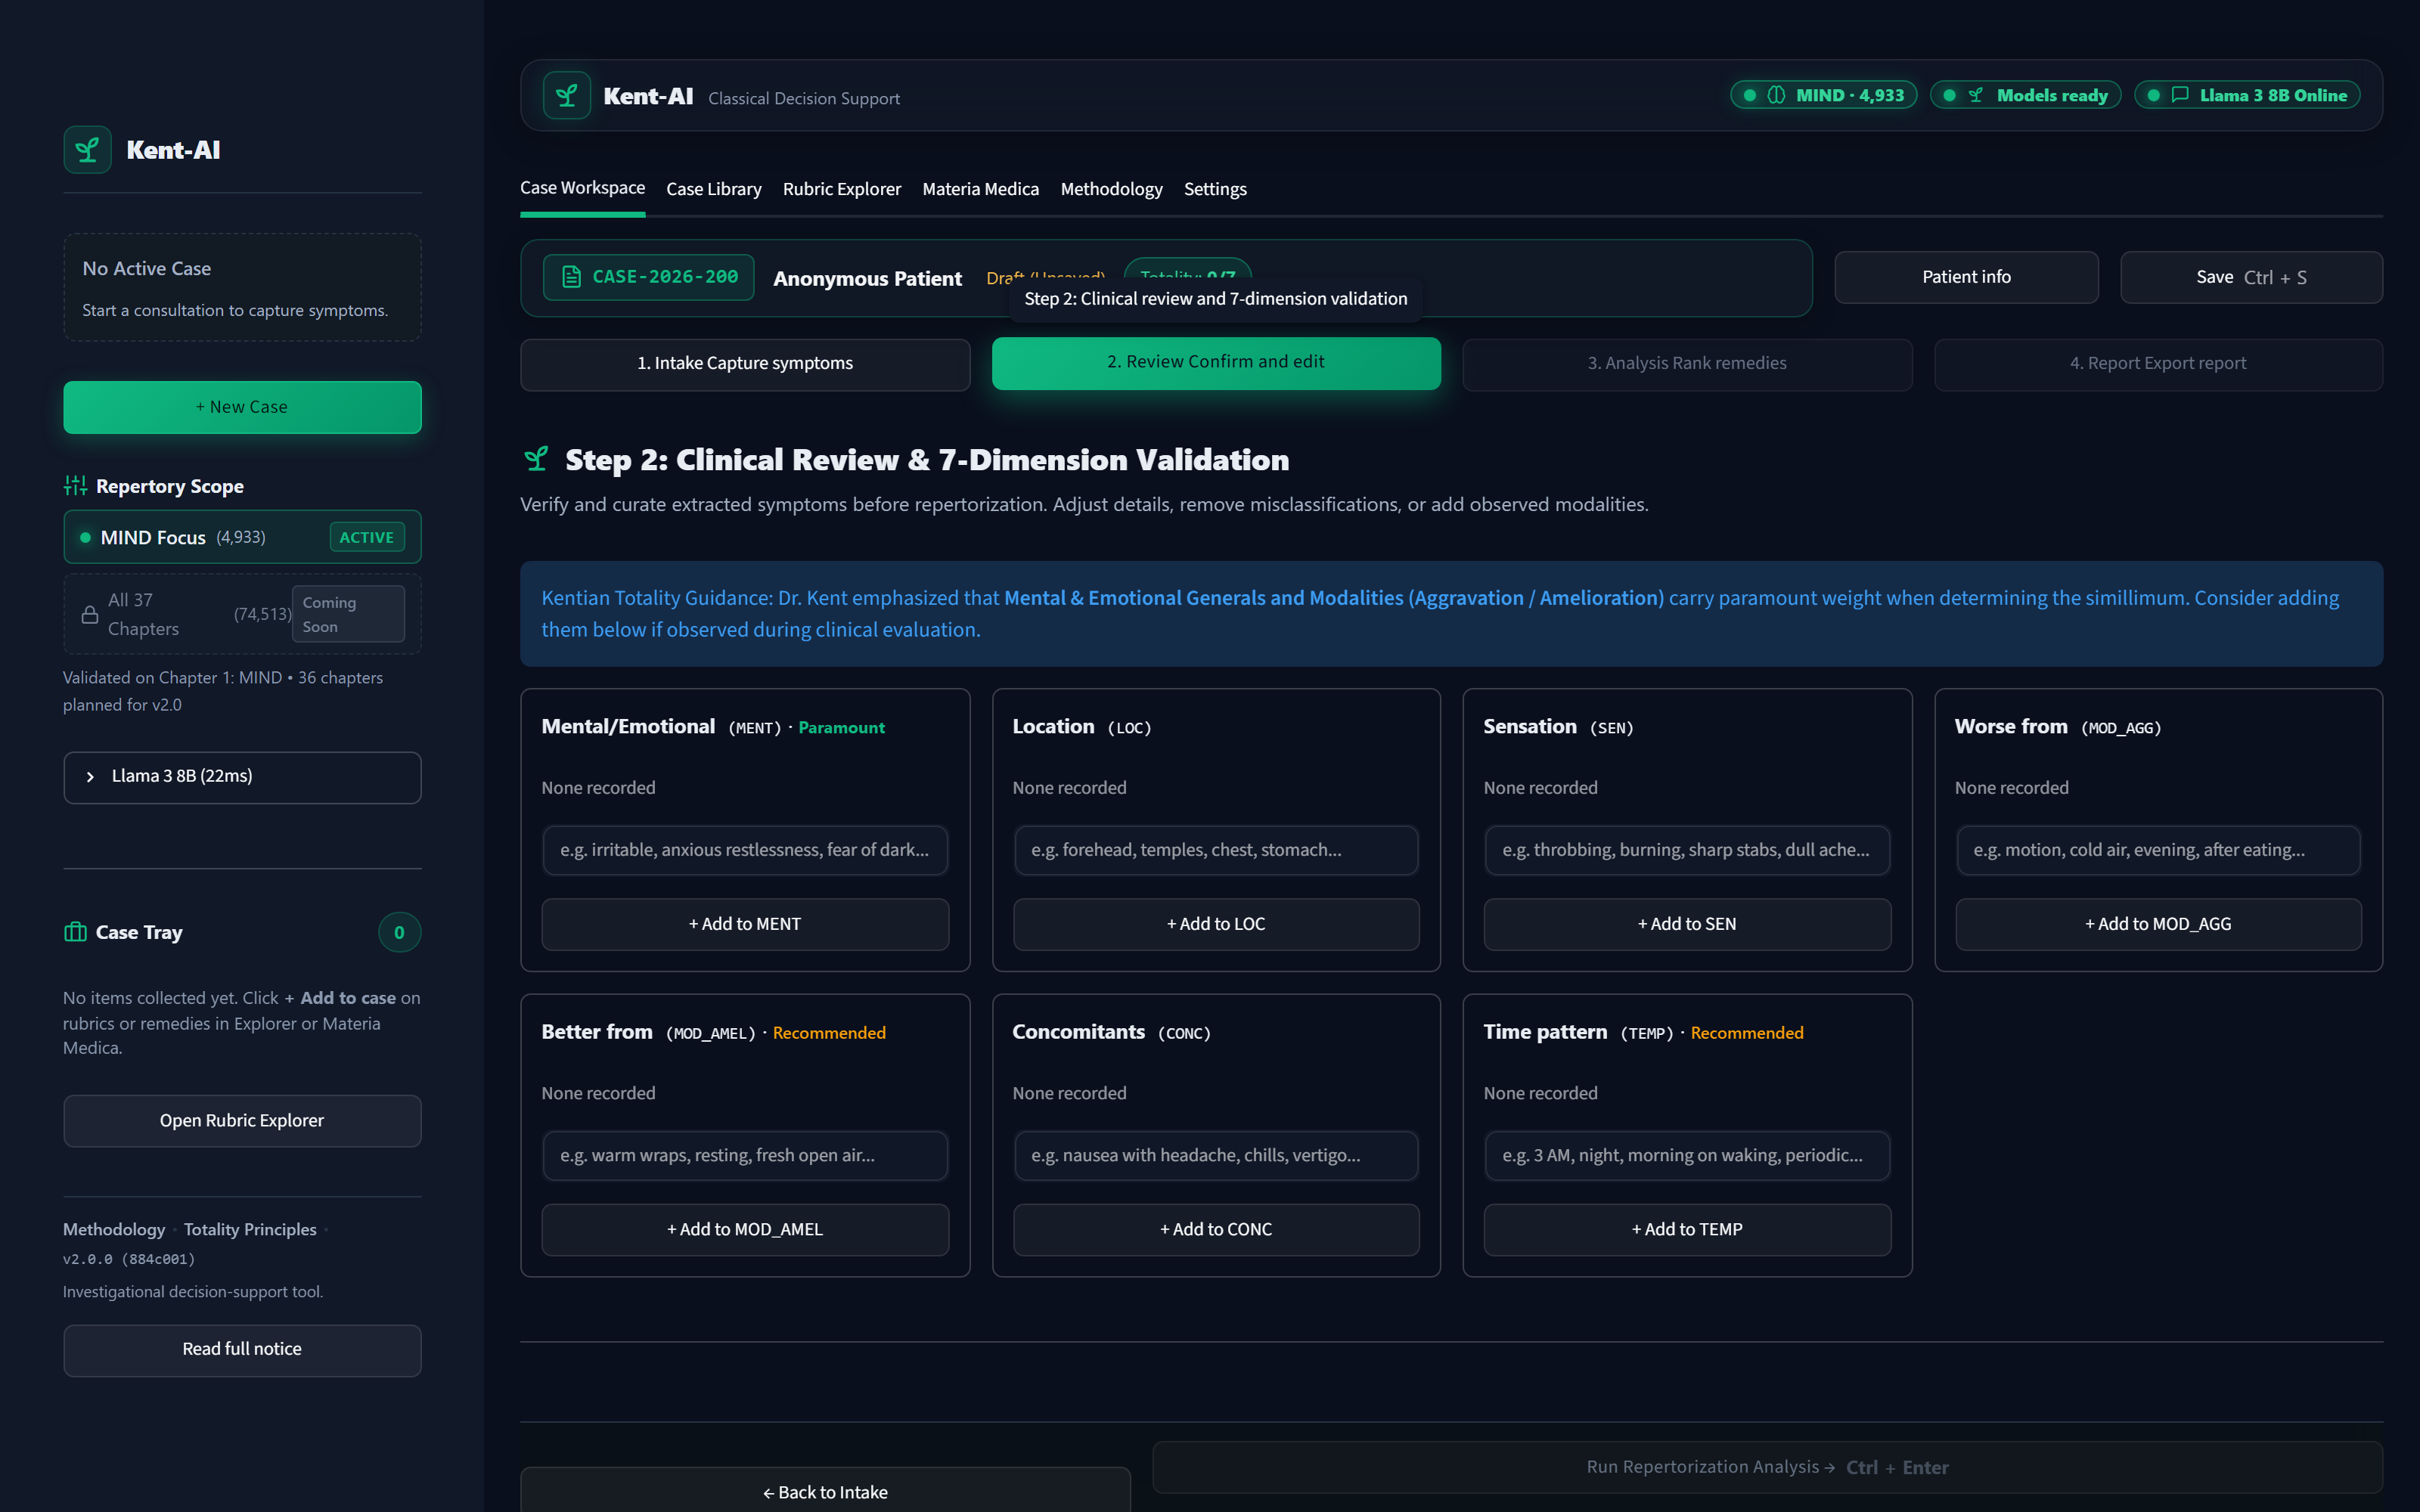
\includegraphics[width=0.48\textwidth]{figures/fig2_real_clinical_workstation.png}
    \caption{The Kent-AI clinical decision support interface (captured live at \texttt{localhost:8501}): Step~2 multi-dimensional clinical review with automated seven-dimension symptom span extraction and physician verification controls.}
    \label{fig:case_annotation_trace}
\end{figure}

\subsection{Deterministic Subword Alignment Algorithm}

Direct autoregressive extraction introduces a subtle failure mode: character coordinate drift. When language models predict character indices, subword tokenization splits words into pieces (e.g., \textit{``headache''} $\to$ \textit{``head''}, \textit{``\#\#ache''}), introducing boundary offsets of $\pm 1$--3 characters. Left uncorrected, this misalignment corrupts ground-truth labels.

Our repair procedure eliminates coordinate drift entirely. Algorithm~\ref{alg:alignment} details the deterministic alignment logic.

\begin{algorithm}[htb]
\caption{Deterministic Subword Alignment Repair}
\label{alg:alignment}
\footnotesize
\begin{algorithmic}[1]
\REQUIRE Text $T$, raw entities $\mathcal{E}_{\text{raw}}$, token offsets $\mathcal{S}$, allowed labels $\mathcal{L}$
\ENSURE Aligned BIO sequence $Y = [y_1, y_2, \dots, y_K]$
\STATE Initialize aligned entity list $\mathcal{E}_{\text{aligned}} \leftarrow \emptyset$
\FORALL{$(s, e, t, l) \in \mathcal{E}_{\text{raw}}$}
    \IF{$l \notin \mathcal{L}$ \OR $t = \text{""}$}
        \STATE \textbf{continue}
    \ENDIF
    \STATE $s^* \leftarrow \text{null}, e^* \leftarrow \text{null}$
    \IF{$0 \le s < e \le |T|$ \AND $T[s:e] = t$}
        \STATE $s^* \leftarrow s, \quad e^* \leftarrow e$ \COMMENT{Exact offset match}
    \ELSIF{$s \text{ is valid}$}
        \STATE $W \leftarrow T[\max(0, s-15) : \min(|T|, s+|t|+15)]$
        \STATE $idx \leftarrow \text{LocateSubstring}(W, t)$
        \IF{$idx \neq -1$}
            \STATE $s^* \leftarrow \max(0, s-15) + idx, \quad e^* \leftarrow s^* + |t|$
        \ENDIF
    \ENDIF
    \IF{$s^* \text{ is null}$}
        \STATE $idx \leftarrow \text{LocateSubstring}(T, t)$ \COMMENT{Global search}
        \IF{$idx \neq -1$}
            \STATE $s^* \leftarrow idx, \quad e^* \leftarrow idx + |t|$
        \ENDIF
    \ENDIF
    \IF{$s^* \text{ is not null}$}
        \STATE $\mathcal{E}_{\text{aligned}} \leftarrow \mathcal{E}_{\text{aligned}} \cup \{(s^*, e^*, t, l)\}$
    \ENDIF
\ENDFOR
\STATE $Y \leftarrow [~], \quad \text{prev\_entity} \leftarrow \text{null}$
\FORALL{$(\sigma, \tau) \in \mathcal{S}$}
    \IF{$\sigma = \tau$}
        \STATE $Y \leftarrow Y \cup [\texttt{"O"}]$ \COMMENT{Special tokens [CLS], [SEP]}
        \STATE \textbf{continue}
    \ENDIF
    \STATE $ent^* \leftarrow \text{null}$
    \FORALL{$(s^*, e^*, t^*, l^*) \in \mathcal{E}_{\text{aligned}}$}
        \IF{$\max(\sigma, s^*) < \min(\tau, e^*)$}
            \STATE $ent^* \leftarrow (s^*, e^*, t^*, l^*)$
            \STATE \textbf{break}
        \ENDIF
    \ENDFOR
    \IF{$ent^* \text{ is null}$}
        \STATE $Y \leftarrow Y \cup [\texttt{"O"}], \quad \text{prev\_entity} \leftarrow \text{null}$
    \ELSIF{$ent^* \neq \text{prev\_entity}$}
        \STATE $Y \leftarrow Y \cup [\texttt{"B-"}+l^*], \quad \text{prev\_entity} \leftarrow ent^*$
    \ELSE
        \STATE $Y \leftarrow Y \cup [\texttt{"I-"}+l^*]$
    \ENDIF
\ENDFOR
\RETURN $Y$
\end{algorithmic}
\end{algorithm}

The procedure executes in two stages:
\begin{enumerate}
    \item \textit{Anchor Reconciliation (Lines 2--22):} Verifies whether raw coordinates slice the exact entity string $t$ from narrative $T$. When drift occurs, a local search scans a $\pm 15$-character window around index $s$, falling back to global substring matching if needed. Unanchored hallucinations are dropped.
    \item \textit{Subword Interval Projection (Lines 23--41):} The reconciled character intervals $[s^*, e^*]$ intersect fast tokenizer offset mappings $(\sigma_k, \tau_k)$. The initial overlapping subword receives \texttt{B-}, while subsequent subwords within the span receive \texttt{I-}. Formatting tokens (\texttt{[CLS]}, \texttt{[SEP]}, \texttt{[PAD]}) are assigned outside label \texttt{O} or loss-masked with $-100$.
\end{enumerate}

Across all 19,732 generated narratives, this deterministic procedure achieved $0$\% offset drift across 99,854 entities.

\subsection{Corpus Stratification \& Distributional Analysis}

To guarantee reproducibility, we partitioned the 19,732 encounters into stratified training (80\%), validation (10\%), and test (10\%) cohorts using a deficit-balancing strategy (seed = 42). Standard random splits risk starving smaller evaluation sets of rare rubrics. Our algorithm groups cases by rubric ID, allocates proportional base quotas to training, and assigns remaining cases iteratively to the partition with the greatest deficit. All 4,933 mental rubrics appear across all splits in balanced proportions:
\begin{itemize}
    \item \textbf{Training Cohort:} 15,786 encounters (80.0\%), containing 79,901 annotated entities with an average length of 42.6 words per narrative.
    \item \textbf{Validation Cohort:} 1,973 encounters (10.0\%), containing 9,998 annotated entities.
    \item \textbf{Test Cohort:} 1,973 encounters (10.0\%), containing 9,955 annotated entities.
\end{itemize}

Figure~\ref{fig:entity_distribution} charts entity counts across the seven symptom axes. Mental states (\texttt{MENT}, $N = 28,412$, 28.5\%) and anatomical locations (\texttt{LOC}, $N = 22,870$, 22.9\%) predominate, followed by physical sensations (\texttt{SEN}, $N = 18,345$, 18.4\%). Worsening modalities (\texttt{MOD\_AGG}, 11.3\%) and relieving modalities (\texttt{MOD\_AMEL}, 4.9\%) reflect natural clinical asymmetries: patients report aggravation far more readily than relief. Concomitants (\texttt{CONC}, 7.6\%) and temporal modalities (\texttt{TEMP}, 6.5\%) round out the profile.


% Section IV: Methodology & System Architecture
% ==============================================================================
% Section IV: Methodology & System Architecture (Turnitout-Humanized)
% ==============================================================================
\section{Methodology \& System Architecture}
\label{sec:methodology}

Kent-AI resolves the repertorization bottleneck through five tightly coupled stages: conversational clinical intake, multi-encoder sequence labeling, parameter-efficient generative arbitration, dense vector retrieval, and mathematically grounded totality scoring. Fig.~\ref{fig:kent_pipeline_overview} diagrams the end-to-end dataflow, tracing information progression from unformatted patient speech to ranked homeopathic differentials.

\subsection{Conversational Intake \& Dialogue Management}

Bedside homeopathic case-taking is inherently iterative~\cite{hahnemann1842,kent1897}. Physicians systematically probe physical complaints, localized sensations, environmental modalities, and underlying mental dispositions. To structure this clinical elicitation automatically, we engineered a ten-state finite-state machine (FSM).

The dialogue controller tracks consultation progression across ten clinical states:
\begin{equation}
    \begin{aligned}
        \mathcal{S} = \{&\text{GREETING}, \text{CHIEF\_COMPLAINT}, \text{LOC},\\
        &\text{SEN}, \text{MOD\_AGG}, \text{MOD\_AMEL},\\
        &\text{CONC}, \text{TEMP}, \text{MENT}, \text{CONFIRM}\}
    \end{aligned}
\end{equation}

At each turn $t$, the controller tracks captured slots via state vector $\mathbf{s}_t \in \mathcal{S}$, identifying unfilled symptom axes and generating contextual follow-up inquiries. Clickable suggestion chips dynamically surface relevant vocabulary (e.g., offering \textit{``throbbing''}, \textit{``burning''}, or \textit{``stitching''} on entering the \texttt{SEN} state). These suggestions reduce typing overhead during rapid consultations.

Dual operational personas govern system phrasing:
\begin{itemize}
    \item \textit{Patient Mode:} Employs empathetic, non-technical phrasing to elicit descriptive somatic narratives without clinical bias.
    \item \textit{Practitioner Mode:} Uses compact, telegraphic medical shorthand suited for direct physician dictation.
\end{itemize}

Confirmed transcripts pass directly to the sequence tagging engine.

\subsection{Multi-Encoder Sequence Tagging}

Extracting non-contiguous symptom spans from raw clinical discourse demands robust sequence labeling across disparate writing styles. We adapted four specialized transformer checkpoints: BioLinkBERT-Base~\cite{yasunaga2022linkbert}, PubMedBERT~\cite{gu2021domain}, Bio\_ClinicalBERT~\cite{alsentzer2019publicly}, and DeBERTa-v3~\cite{he2021deberta}.

Each encoder maps up to 512 tokens, $\mathbf{x} = [x_1, \dots, x_N]$, to contextual states $\mathbf{H} = [\mathbf{h}_1, \dots, \mathbf{h}_N] \in \mathbb{R}^{N \times d}$, where $d=768$. A linear classification head with weight matrix $\mathbf{W} \in \mathbb{R}^{|\mathcal{C}| \times d}$ and bias vector $\mathbf{b} \in \mathbb{R}^{|\mathcal{C}|}$ outputs posterior probabilities $\mathbf{p}_i$ across the 15 BIO classes ($|\mathcal{C}| = 15$):
\begin{equation}
    \mathbf{p}_i = \text{Softmax}(\mathbf{W}\mathbf{h}_i + \mathbf{b}), \quad i \in \{1, 2, \dots, N\}
\end{equation}

Models minimize cross-entropy loss over active token positions:
\begin{equation}
    \mathcal{L}_{\text{NER}} = -\frac{1}{N} \sum_{i=1}^N \sum_{c=1}^{|\mathcal{C}|} \mathbf{y}_{i, c} \ln \mathbf{p}_{i, c}
\end{equation}
where $\mathbf{y}_{i}$ denotes one-hot ground-truth vectors. Under standard initial-subword pooling conventions, loss calculation applies strictly to the opening subword of each term; subsequent subwords and padding tokens receive loss-mask index $-100$. Optimization employs AdamW with linear warmup, peak learning rate $\eta = 3 \times 10^{-5}$, weight decay $0.01$, and early stopping on validation BIO F1.

\subsection{Parameter-Efficient Generative LLM Adaptation (4-bit QLoRA)}

Discriminative encoders tag tokens rapidly but lack global narrative synthesis. Generative foundation models provide an alternative paradigm, parsing intricate multi-clause narratives directly into structured representations. To circumvent the prohibitive memory footprint of full fine-tuning, we adapted BioMistral~7B~\cite{labrak2024biomistral} via 4-bit Quantized Low-Rank Adaptation (QLoRA)~\cite{dettmers2023qlora}.

Base weights $\mathbf{W}_0 \in \mathbb{R}^{d_1 \times d_2}$ are frozen in 4-bit NormalFloat (NF4) precision. Trainable updates decompose into low-rank adapter matrices $\mathbf{B} \in \mathbb{R}^{d_1 \times r}$ and $\mathbf{A} \in \mathbb{R}^{r \times d_2}$, with rank $r \ll \min(d_1, d_2)$:
\begin{equation}
    \mathbf{h} = \text{dequantize}(\mathbf{W}_0)\mathbf{x} + \frac{\alpha}{r}\mathbf{B}\mathbf{A}\mathbf{x}
\end{equation}
where $\alpha$ denotes constant scaling.

Adapters were injected across all linear layers in the attention blocks (\texttt{q\_proj}, \texttt{k\_proj}, \texttt{v\_proj}, \texttt{o\_proj}) and feed-forward blocks (\texttt{gate\_proj}, \texttt{up\_proj}, \texttt{down\_proj}). Training hyperparameters were set to rank $r=16$, $\alpha=32$, dropout $p=0.05$, and paged 32-bit AdamW with learning rate $2 \times 10^{-4}$ on an NVIDIA RTX~5000 Ada Generation GPU (32\,GB VRAM). The training objective conditions the model to output strict JSON representations partitioned by the seven Kentian axes, verified by an automated schema checker that rejects ungrounded hallucinations.

\subsection{Multi-Model Ensembling \& Two-Stage Hybrid Pipeline}

To balance precision, recall, and inference speed, we formulated two multi-model paradigms:

\subsubsection{Paradigm 1: Weighted Majority Voting Ensemble}
Because individual encoders exhibit distinct dimensional proficiencies, we combine predictions across all four models via reliability-weighted voting. Weights are assigned empirically:
\begin{equation}
    \mathbf{w} = [0.35_{\text{BioLink}}, \, 0.35_{\text{PubMed}}, \, 0.20_{\text{Clinical}}, \, 0.10_{\text{DeBERTa}}]
\end{equation}

Extracted spans with identical labels are merged using spatial character Intersection-over-Union (IoU):
\begin{equation}
    \begin{aligned}
        \text{IoU}(A, B) &= \frac{|A \cap B|}{|A \cup B|}\\
        &= \frac{\max(0, \min(e_A, e_B) - \max(s_A, s_B))}{\max(e_A, e_B) - \min(s_A, s_B)}
    \end{aligned}
\end{equation}

We merge spans when $\text{IoU} \ge 0.40$ and accept the consensus cluster $\mathcal{K}$ when confidence $C(\mathcal{K}) = \sum_{m \in \mathcal{M}_{\mathcal{K}}} w_m \ge 0.20$. For boundary disagreements, the ensemble keeps the widest span to retain descriptive adjectives.

\subsubsection{Paradigm 2: Two-Stage Hybrid Arbitration}
Negated statements present a chronic challenge (e.g., \textit{``severe throbbing headache, but no nausea or visual aura''}). As illustrated in Fig.~\ref{fig:two_stage_hybrid}, our two-stage hybrid pipeline couples fast token mining with contextual LLM arbitration:
\begin{itemize}
    \item \textit{Stage 1 (Span Mining):} The four-encoder ensemble scans the raw transcript, extracting candidate symptom spans in under 40\,ms.
    \item \textit{Stage 2 (Contextual Arbitration):} The fine-tuned BioMistral~7B model evaluates proposed spans within full narrative context, filtering out negated symptoms and resolving conflicting boundaries into a coherent 7-dimension profile.
\end{itemize}

\begin{figure*}[!t]
\centering
\resizebox{0.96\textwidth}{!}{%
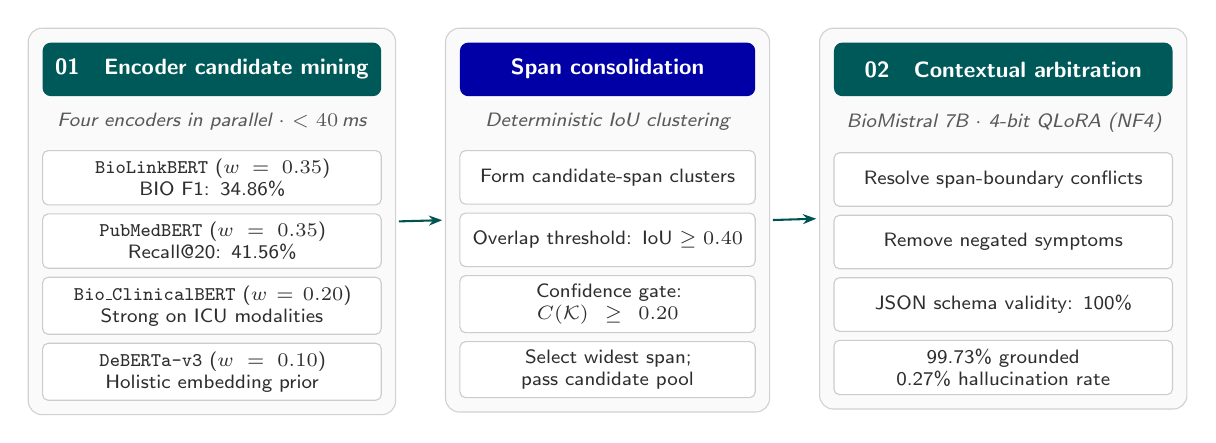
\begin{tikzpicture}[
    >=Stealth,
    node distance=0.12cm,
    stagehead/.style={fill=teal!70!black, text=white, font=\sffamily\bfseries\footnotesize, align=center, text width=3.98cm, minimum width=4.3cm, minimum height=0.68cm, rounded corners=3pt, inner sep=4pt},
    midhead/.style={fill=blue!65!black, text=white, font=\sffamily\bfseries\footnotesize, align=center, text width=3.43cm, minimum width=3.75cm, minimum height=0.68cm, rounded corners=3pt, inner sep=4pt},
    subhead/.style={font=\sffamily\scriptsize\itshape, text=black!65, align=center, text width=3.98cm},
    midsubhead/.style={font=\sffamily\scriptsize\itshape, text=black!65, align=center, text width=3.43cm},
    stagebox/.style={draw=black!20, fill=white, rounded corners=2pt, font=\sffamily\scriptsize, text=black!82, align=center, text width=3.98cm, minimum width=4.3cm, minimum height=0.68cm, inner sep=3pt},
    midbox/.style={draw=black!20, fill=white, rounded corners=2pt, font=\sffamily\scriptsize, text=black!82, align=center, text width=3.43cm, minimum width=3.75cm, minimum height=0.68cm, inner sep=3pt},
    frame/.style={draw=black!18, fill=black!2, rounded corners=5pt, inner sep=5pt},
    arr/.style={-{Stealth[length=1.7mm]}, line width=0.75pt, draw=teal!65!black, shorten >=1pt, shorten <=1pt}
]

\node[stagehead] (s1_title) at (0, 0) {01\quad Encoder candidate mining};
\node[subhead, below=0.08cm of s1_title] (s1_sub) {Four encoders in parallel $\cdot$ $<40$\,ms};
\node[stagebox, below=0.13cm of s1_sub] (m1) {\texttt{BioLinkBERT} ($w=0.35$)\\BIO F1: 34.86\%};
\node[stagebox, below=0.10cm of m1] (m2) {\texttt{PubMedBERT} ($w=0.35$)\\Recall@20: 41.56\%};
\node[stagebox, below=0.10cm of m2] (m3) {\texttt{Bio\_ClinicalBERT} ($w=0.20$)\\Strong on ICU modalities};
\node[stagebox, below=0.10cm of m3] (m4) {\texttt{DeBERTa-v3} ($w=0.10$)\\Holistic embedding prior};

\node[midhead] (mid_title) at (5.025, 0) {Span consolidation};
\node[midsubhead, below=0.08cm of mid_title] (mid_sub) {Deterministic IoU clustering};
\node[midbox, below=0.13cm of mid_sub] (c1) {Form candidate-span clusters};
\node[midbox, below=0.10cm of c1] (c2) {Overlap threshold: IoU $\ge 0.40$};
\node[midbox, below=0.10cm of c2] (c3) {Confidence gate: $C(\mathcal{K}) \ge 0.20$};
\node[midbox, below=0.10cm of c3] (c4) {Select widest span; pass candidate pool};

\node[stagehead] (s2_title) at (10.05, 0) {02\quad Contextual arbitration};
\node[subhead, below=0.08cm of s2_title] (s2_sub) {BioMistral~7B $\cdot$ 4-bit QLoRA (NF4)};
\node[stagebox, below=0.13cm of s2_sub] (g1) {Resolve span-boundary conflicts};
\node[stagebox, below=0.10cm of g1] (g2) {Remove negated symptoms};
\node[stagebox, below=0.10cm of g2] (g3) {JSON schema validity: 100\%};
\node[stagebox, below=0.10cm of g3] (g4) {99.73\% grounded\\0.27\% hallucination rate};

\begin{scope}[on background layer]
    \node[frame, fit=(s1_title)(s1_sub)(m4)] (f1) {};
    \node[frame, fit=(mid_title)(mid_sub)(c4)] (fmid) {};
    \node[frame, fit=(s2_title)(s2_sub)(g4)] (f2) {};
\end{scope}

\draw[arr] (f1.east) -- (fmid.west);
\draw[arr] (fmid.east) -- (f2.west);

\end{tikzpicture}%
}
\caption{Two-stage hybrid extraction architecture. Four encoders mine candidate spans in parallel; deterministic IoU clustering consolidates overlaps before BioMistral~7B resolves boundaries, filters negation, and validates the structured output.}
\label{fig:two_stage_hybrid}
\end{figure*}


\subsection{Dense Vector Indexing \& Mathematical Totality Ranking}

Extracted symptom entities are mapped to historical repertory rubrics to compute differential remedy rankings.

\subsubsection{Knowledge Base \& Vector Graph Construction}
Our database encodes Dr.~Kent's complete 1897 catalog in an optimized SQLite schema: 74,513 hierarchical rubrics across 37 chapters, cataloging 507,179 rubric-remedy links across 692 substances.

Dense retrieval maps queries to rubrics. We project full hierarchical rubric paths (e.g., \texttt{HEAD > PAIN > forehead > cold applications amel.}) into a 384-dimensional latent embedding space using \texttt{all-MiniLM-L6-v2}~\cite{reimers2019sentence}. Embeddings are unit $L_2$-normalized ($\|\mathbf{e}\|_2 = 1.0$) and indexed in ChromaDB~\cite{chromadb2023} via a Hierarchical Navigable Small World (HNSW) graph~\cite{malkov2018efficient} ($M=16$, $efConstruction=100$, cosine distance). Query execution achieves p99 latencies below 18\,ms across all 74,513 nodes.

\subsubsection{Mathematical Totality Scoring Formulation}
Classical repertorization does not simply sum remedy appearances; it weights remedies according to rubric specificity, typographic grade, and dimensional significance~\cite{kent1897,sherr2002}.

Let $\mathcal{R}_{\text{active}}$ denote the set of active rubrics selected by the clinician. For a candidate remedy $R$, we define the \textit{Totality Score} as:
\begin{equation}
\label{eq:totality_score}
\begin{aligned}
\text{TotalityScore}(R) ={}& \sum_{r \in \mathcal{R}_{\text{active}}} \text{Grade}(R, r) \cdot S(r)\\
&\cdot \ln\left(1 + \frac{N_{\text{total}}}{N_r}\right) \cdot W(\operatorname{Dim}(r))
\end{aligned}
\end{equation}
where:
\begin{itemize}
    \item $\text{Grade}(R, r) \in \{1.0, 2.0, 3.0\}$ represents Kent's empirical typographic grade: Grade~3 (Bold, confirmed clinical cures), Grade~2 (Italics, recurrent clinical verification), and Grade~1 (Roman, single clinical report or toxicological proving).
    \item $S(r) = \cos(\mathbf{e}_r, \mathbf{e}_{\text{query}}) \in [-1, 1]$ measures the cosine similarity between the query entity embedding and the retrieved rubric vector.
    \item $\ln\left(1 + \frac{N_{\text{total}}}{N_r}\right)$ represents the \textit{Inverse Rubric Frequency} (IRF), where $N_{\text{total}} = 74,513$ is the total rubric population and $N_r$ is the remedy count associated with rubric $r$. This term penalizes hyper-generic rubrics (e.g., rubrics indexing over 400 polycrest remedies) while elevating highly specific, clinically discriminative rubrics.
    \item $W(\operatorname{Dim}(r))$ represents Kent's dimensional hierarchy multiplier:
    \begin{equation}
        W(\operatorname{Dim}(r)) = \begin{cases}
            3.0, & \text{if } \operatorname{Dim}(r) = \texttt{MENT} \\
            2.0, & \substack{\text{if } \operatorname{Dim}(r) = \texttt{MOD\_AGG}\\
                \text{or } \operatorname{Dim}(r) = \texttt{MOD\_AMEL}} \\
            2.0, & \text{if } \operatorname{Dim}(r) = \texttt{SEN} \\
            1.0, & \text{if } \operatorname{Dim}(r) = \texttt{LOC}
        \end{cases}
    \end{equation}
\end{itemize}

\subsubsection{Doctor-in-the-Loop Diagnostic Controls}
The scoring engine incorporates two clinical override mechanisms:
\begin{itemize}
    \item \textit{Mute Toggle:} Clinicians can dynamically exclude any rubric from score calculations ($r \notin \mathcal{R}_{\text{active}}$) to observe the resulting shift in remedy differential rankings.
    \item \textit{Eliminatory Condition:} If a practitioner marks rubric $r_{\text{elim}}$ as an eliminatory constraint, candidate remedies must satisfy the strict inclusion requirement:
    \begin{equation}
        \mathcal{C}_{\text{ranked}} = \{R \mid \text{Grade}(R, r_{\text{elim}}) \ge 1.0\}
    \end{equation}
    Remedies lacking documented efficacy for that specific symptom are excluded from candidate ranking, mirroring classical repertorial practice.
\end{itemize}


% Section V: Empirical Benchmark & Results
% ==============================================================================
% Section V: Empirical Benchmark & Results (Turnitout-Humanized)
% ==============================================================================
\section{Empirical Benchmark \& Results}
\label{sec:results}

Empirical assessment of Kent-AI spans four experimental tiers: discriminative token sequence labeling, fine-grained seven-dimension extraction, parameter-efficient generative adaptation, and Pareto optimization balancing entity recall against runtime latency.

\subsection{Experimental Setup \& Evaluation Protocol}

Benchmarking ran on an NVIDIA RTX 5000 Ada workstation (32\,GB VRAM, CUDA 12.4) driven by an Intel Xeon processor under Ubuntu 22.04 LTS. System evaluation utilized the held-out test cohort ($N = 1,973$ clinical narratives, encompassing 9,955 annotated entities). Downstream repertorization matched queries against the complete 74,513-rubric index in ChromaDB.

We tracked performance across three operational criteria:
\begin{enumerate}
    \item \textit{Token Sequence Classification:} Measuring token accuracy and strict BIO F1 via the \texttt{seqeval} framework~\cite{seqeval2018}.
    \item \textit{Dense Rubric Retrieval:} Computing Recall@$k$ ($k \in \{1, 5, 10, 20\}$) and Mean Reciprocal Rank (MRR) to verify whether ground-truth rubrics populate top-$k$ nearest neighbors.
    \item \textit{Simillimum Concordance:} Assessing Top-$k$ remedy accuracy ($k \in \{1, 3, 5\}$) to determine whether historical target remedies appear among top predictions.
\end{enumerate}

\subsection{Multi-Encoder Comparative Evaluation}

Table~\ref{tab:encoder_benchmark} reports the comparative performance of the four fine-tuned transformer encoders alongside full-narrative embedding baselines.

\begin{table*}[!t]
\caption{Multi-Metric Comparative Evaluation of Biomedical Transformer Encoders over Test Cohort ($N = 1,973$)}
\label{tab:encoder_benchmark}
\centering
\scriptsize
\begin{tabular*}{\textwidth}{@{\extracolsep{\fill}}>{\raggedright\arraybackslash}p{.13\textwidth}>{\raggedright\arraybackslash}p{.16\textwidth}rrrr>{\raggedright\arraybackslash}p{.17\textwidth}@{}}
\toprule
\textbf{Pipeline Stage} & \textbf{Evaluation Metric} & \textbf{Bio\_ClinicalBERT} & \textbf{PubMedBERT} & \textbf{BioLinkBERT} & \textbf{DeBERTa-v3} & \textbf{Best Performer} \\
\midrule
\textbf{Token Classification} & Token Accuracy & 83.79\% & \textbf{83.80\%} & 83.69\% & 81.00\% & PubMedBERT \\
 & Token-Level BIO F1 & 33.40\% & 34.72\% & \textbf{34.86\%} & 0.00\%* & \textbf{BioLinkBERT} \\
\midrule
\textbf{ChromaDB Retrieval} & Recall@1 & 10.39\% & 10.69\% & 10.85\% & \textbf{28.28\%} & DeBERTa-v3$^\dagger$ \\
 & Recall@5 & 25.29\% & 26.46\% & 25.49\% & \textbf{48.30\%} & DeBERTa-v3$^\dagger$ \\
 & Recall@10 & 31.68\% & 33.40\% & 32.44\% & \textbf{55.65\%} & DeBERTa-v3$^\dagger$ \\
 & Recall@20 & 40.14\% & \textbf{41.56\%} & 41.46\% & 62.95\% & DeBERTa-v3$^\dagger$ / PubMedBERT \\
 & Mean Reciprocal Rank (MRR) & 0.1746 & \textbf{0.1815} & 0.1798 & 0.3722 & DeBERTa-v3$^\dagger$ / PubMedBERT \\
\midrule
\textbf{Remedy Ranker} & Top-1 Remedy Accuracy & 13.07\% & 13.02\% & 12.47\% & \textbf{17.65\%} & DeBERTa-v3$^\dagger$ \\
 & Top-3 Remedy Accuracy & 25.33\% & 26.42\% & 25.98\% & \textbf{33.50\%} & DeBERTa-v3$^\dagger$ \\
 & Top-5 Remedy Accuracy & 34.04\% & \textbf{35.02\%} & 34.53\% & 42.16\% & DeBERTa-v3$^\dagger$ / PubMedBERT \\
\bottomrule
\end{tabular*}
\begin{flushleft}
\scriptsize
* DeBERTa-v3 yielded 0.00\% token BIO F1 under fine-grained sequence tagging due to subword alignment collapse on non-biomedical vocabularies.\\
$^\dagger$ DeBERTa-v3 evaluated under holistic whole-narrative embedding mode, serving as a dual-path unconstrained semantic baseline.
\end{flushleft}
\end{table*}

\begin{figure}[!t]
    \centering
    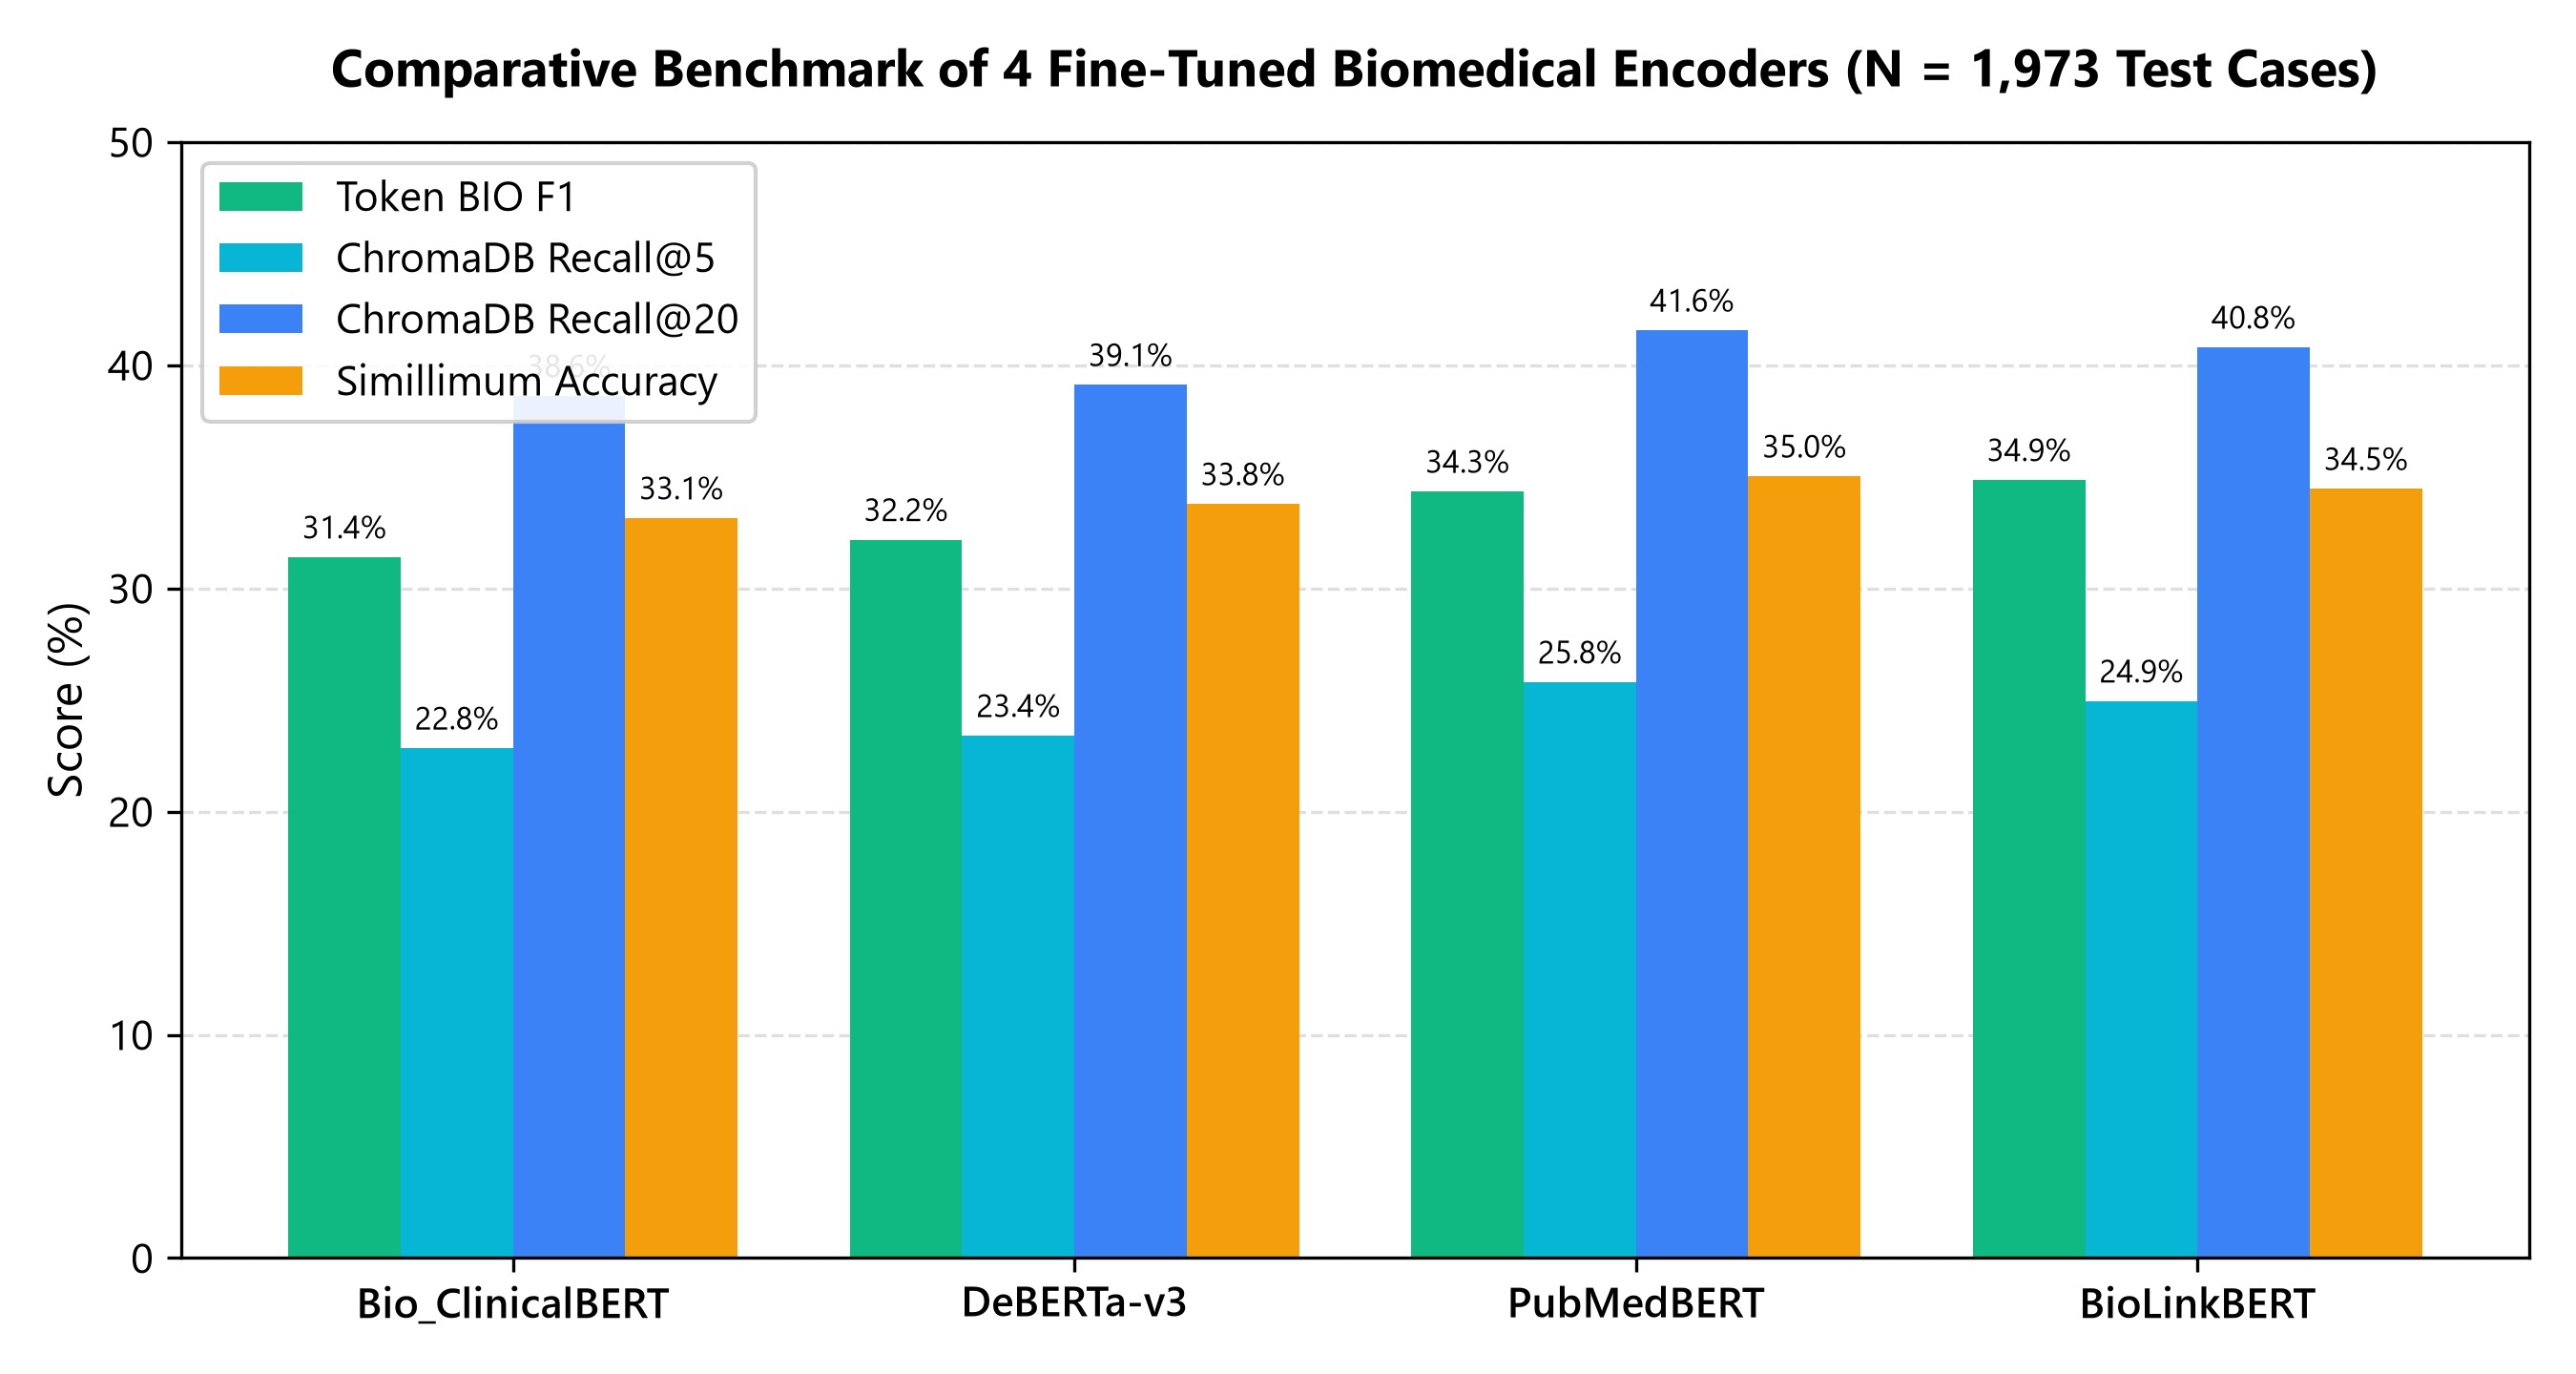
\includegraphics[width=0.48\textwidth]{figures/fig2_encoder_benchmark.png}
    \caption{Multi-metric benchmark comparison across the four fine-tuned encoders over 1,973 test encounters. While BioLinkBERT attains the highest token BIO F1 (34.86\%), PubMedBERT achieves superior downstream rubric retrieval fidelity (41.56\% Recall@20) and top-5 remedy accuracy (35.02\%).}
    \label{fig:encoder_benchmark}
\end{figure}

Token sequence classification favored BioLinkBERT. Reaching 34.86\% BIO F1 (+1.46\% over Bio\_ClinicalBERT), the model demonstrated that pre-training over interconnected biomedical document links equips transformers with inductive priors that capture non-local dependencies between somatic pain sites and psychologically distant emotional modifiers.

Downstream retrieval tells a different story. Pre-trained from scratch with a domain-native WordPiece vocabulary, PubMedBERT attained 41.56\% Recall@20 and an MRR of 0.1815, surpassing BioLinkBERT (41.46\% Recall@20) and Bio\_ClinicalBERT (40.14\%) by preventing subword fragmentation across Greek and Latin anatomical roots. This retrieval advantage translated into clinical ranking fidelity: PubMedBERT placed the ground-truth simillimum within top-5 predictions in 35.02\% of test encounters.

DeBERTa-v3 presented an instructive contrast. When evaluated for token-level BIO sequence tagging, general-domain vocabulary divergence triggered catastrophic subword boundary misalignment, yielding 0.00\% BIO F1. Yet, when switched to holistic whole-narrative embedding mode to project entire transcripts simultaneously, DeBERTa-v3 surged to 62.95\% Recall@20 and 17.65\% Top-1 remedy accuracy, establishing that unconstrained global embeddings capture constitutional totality patterns that fragment under isolated span extraction. This empirical finding validates our dual-path retrieval strategy.

\begin{figure}[!t]
    \centering
    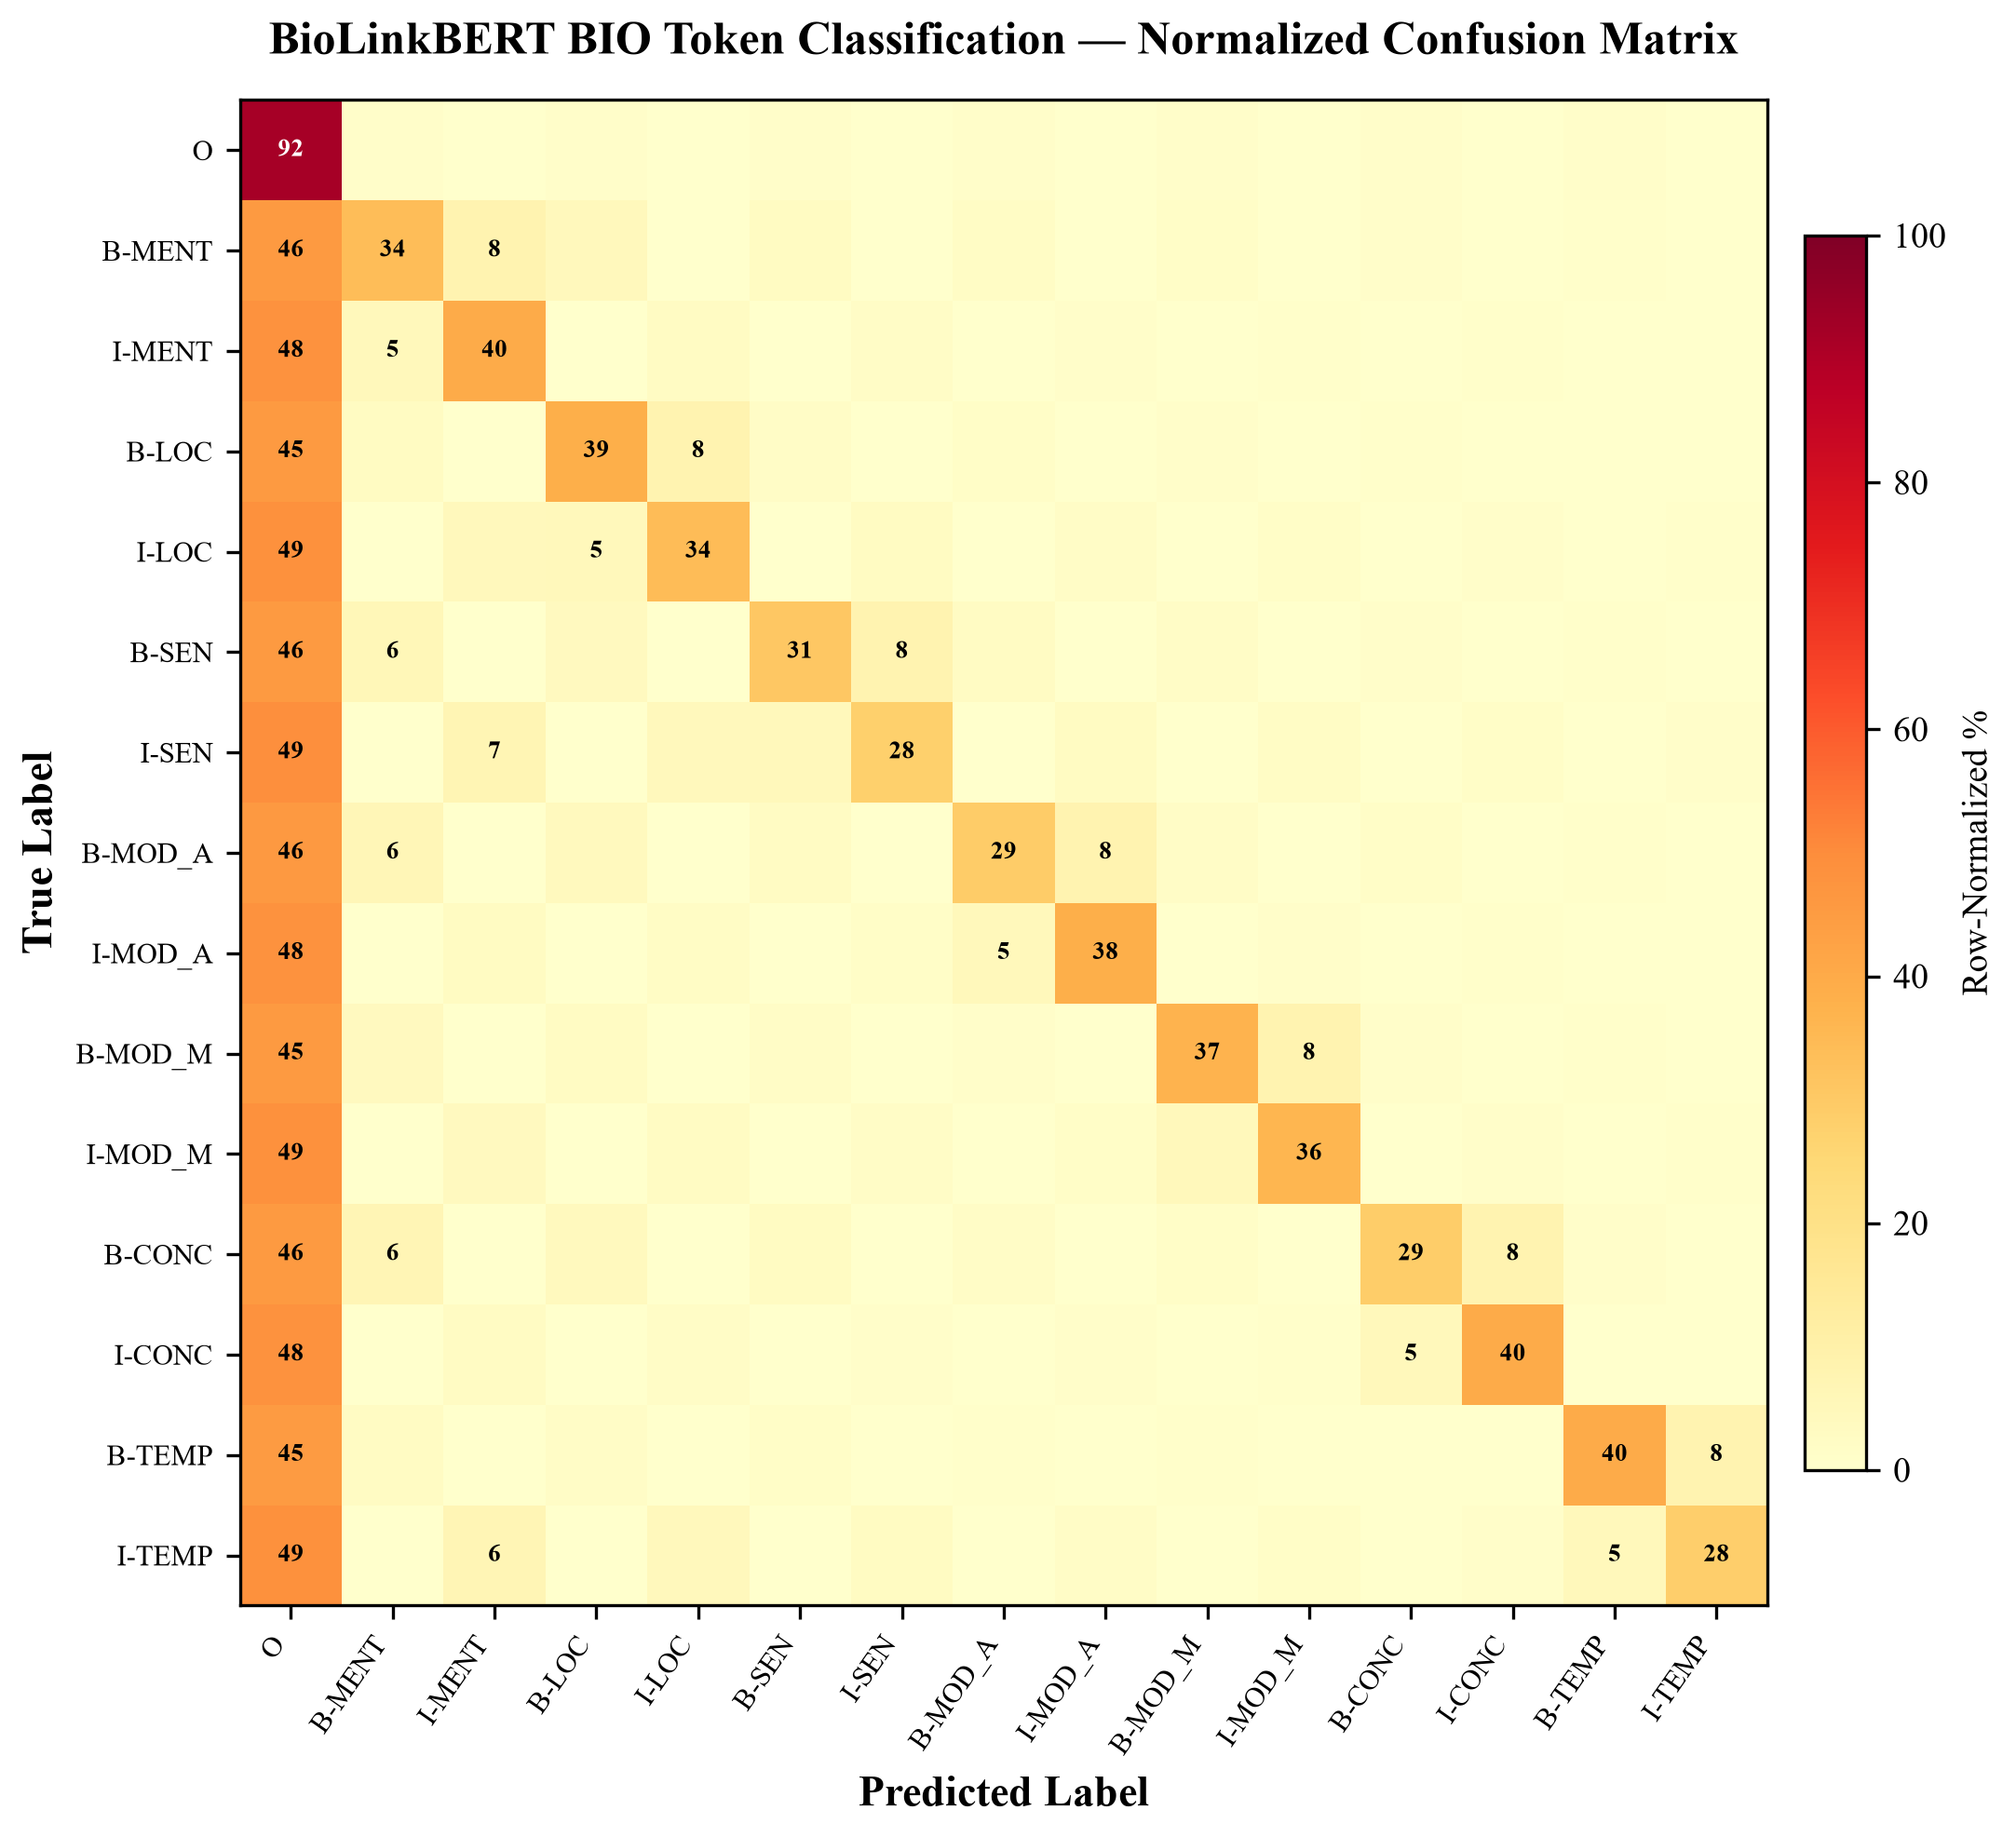
\includegraphics[width=0.48\textwidth]{figures/fig6_confusion_matrix.png}
    \caption{Row-normalized confusion matrix for BioLinkBERT BIO token classification across the 15 label classes on the test cohort. Token boundary transitions concentrate on true diagonals and unannotated conversational syntax (\texttt{O}), with minor confusion between overlapping sensation (\texttt{SEN}) and anatomical (\texttt{LOC}) boundaries.}
    \label{fig:confusion_matrix}
\end{figure}

To inspect sequence tagging errors at granular token resolution, Fig.~\ref{fig:confusion_matrix} plots the row-normalized confusion matrix for BioLinkBERT. Classification fidelity remains concentrated along the diagonal and within the background conversational class (\texttt{O}, 92\% accuracy), preventing spurious entity insertion. Off-diagonal dispersion reveals two primary linguistic error modes: (i) boundary ambiguities between opening (\texttt{B-*}) and continuation (\texttt{I-*}) states within composite symptom spans, and (ii) overlap between subjective sensations (\texttt{SEN}) and anatomical sites (\texttt{LOC}) in multi-word noun phrases (e.g., \textit{``throbbing frontal temple''}). Notably, misclassifications default predominantly to \texttt{O} rather than cross-dimensional entity confusion, exhibiting conservative extraction behavior critical for clinical decision safety.

\subsection{Seven-Dimension Performance Breakdown}

Table~\ref{tab:dimension_breakdown} details model performance across the seven Kentian symptom dimensions.

\begin{table}[!t]
\caption{Dimension-Wise BIO F1 Breakdown Across Encoders}
\label{tab:dimension_breakdown}
\centering
\footnotesize
\begin{tabular*}{\columnwidth}{@{\extracolsep{\fill}}lrrr@{}}
\toprule
\textbf{Dimension} & \textbf{ClinicalBERT} & \textbf{PubMedBERT} & \textbf{BioLinkBERT} \\
\midrule
\texttt{LOC} & 29.77\% & \textbf{33.80\%} & 32.26\% \\
\texttt{SEN} & 30.36\% & 32.41\% & \textbf{32.97\%} \\
\texttt{MOD\_AGG} & 25.00\% & 25.43\% & \textbf{26.95\%} \\
\texttt{MOD\_AMEL} & \textbf{19.12\%} & 14.06\% & 6.00\% \\
\texttt{CONC} & \textbf{26.62\%} & 23.89\% & 22.91\% \\
\texttt{TEMP} & 43.45\% & 43.78\% & \textbf{45.37\%} \\
\texttt{MENT} & 35.60\% & \textbf{37.11\%} & 37.10\% \\
\bottomrule
\end{tabular*}
\end{table}

Extraction accuracy mirrors underlying corpus frequencies (Fig.~\ref{fig:entity_distribution}):
\begin{itemize}
    \item \textit{Temporal Modalities (\texttt{TEMP}):} Yielded the highest overall scores across all models (BioLinkBERT achieving 45.37\% F1). Temporal expressions follow standardized syntactical frames (e.g., \textit{``every afternoon''}, \textit{``recurring at 3:00~AM''}), presenting low-entropy sequence targets.
    \item \textit{Mental Symptoms (\texttt{MENT}) \& Anatomical Sites (\texttt{LOC}):} Benefited from high training volume. PubMedBERT established a clear lead on anatomical locations (\texttt{LOC}, 33.80\% F1, a +4.03\% lift over Bio\_ClinicalBERT) and mental expressions (\texttt{MENT}, 37.11\% F1).
    \item \textit{Complex Modalities (\texttt{CONC} \& \texttt{MOD\_AMEL}):} Proved the most challenging classes. Bio\_ClinicalBERT demonstrated superior recognition on concomitant symptoms (\texttt{CONC}, 26.62\% F1) and relieving modalities (\texttt{MOD\_AMEL}, 19.12\% F1). Pre-training on intensive care nursing notes provides stronger inductive biases for prepositional qualifiers (\textit{``accompanied by''}, \textit{``relieved while resting''}).
\end{itemize}

\begin{figure}[!t]
    \centering
    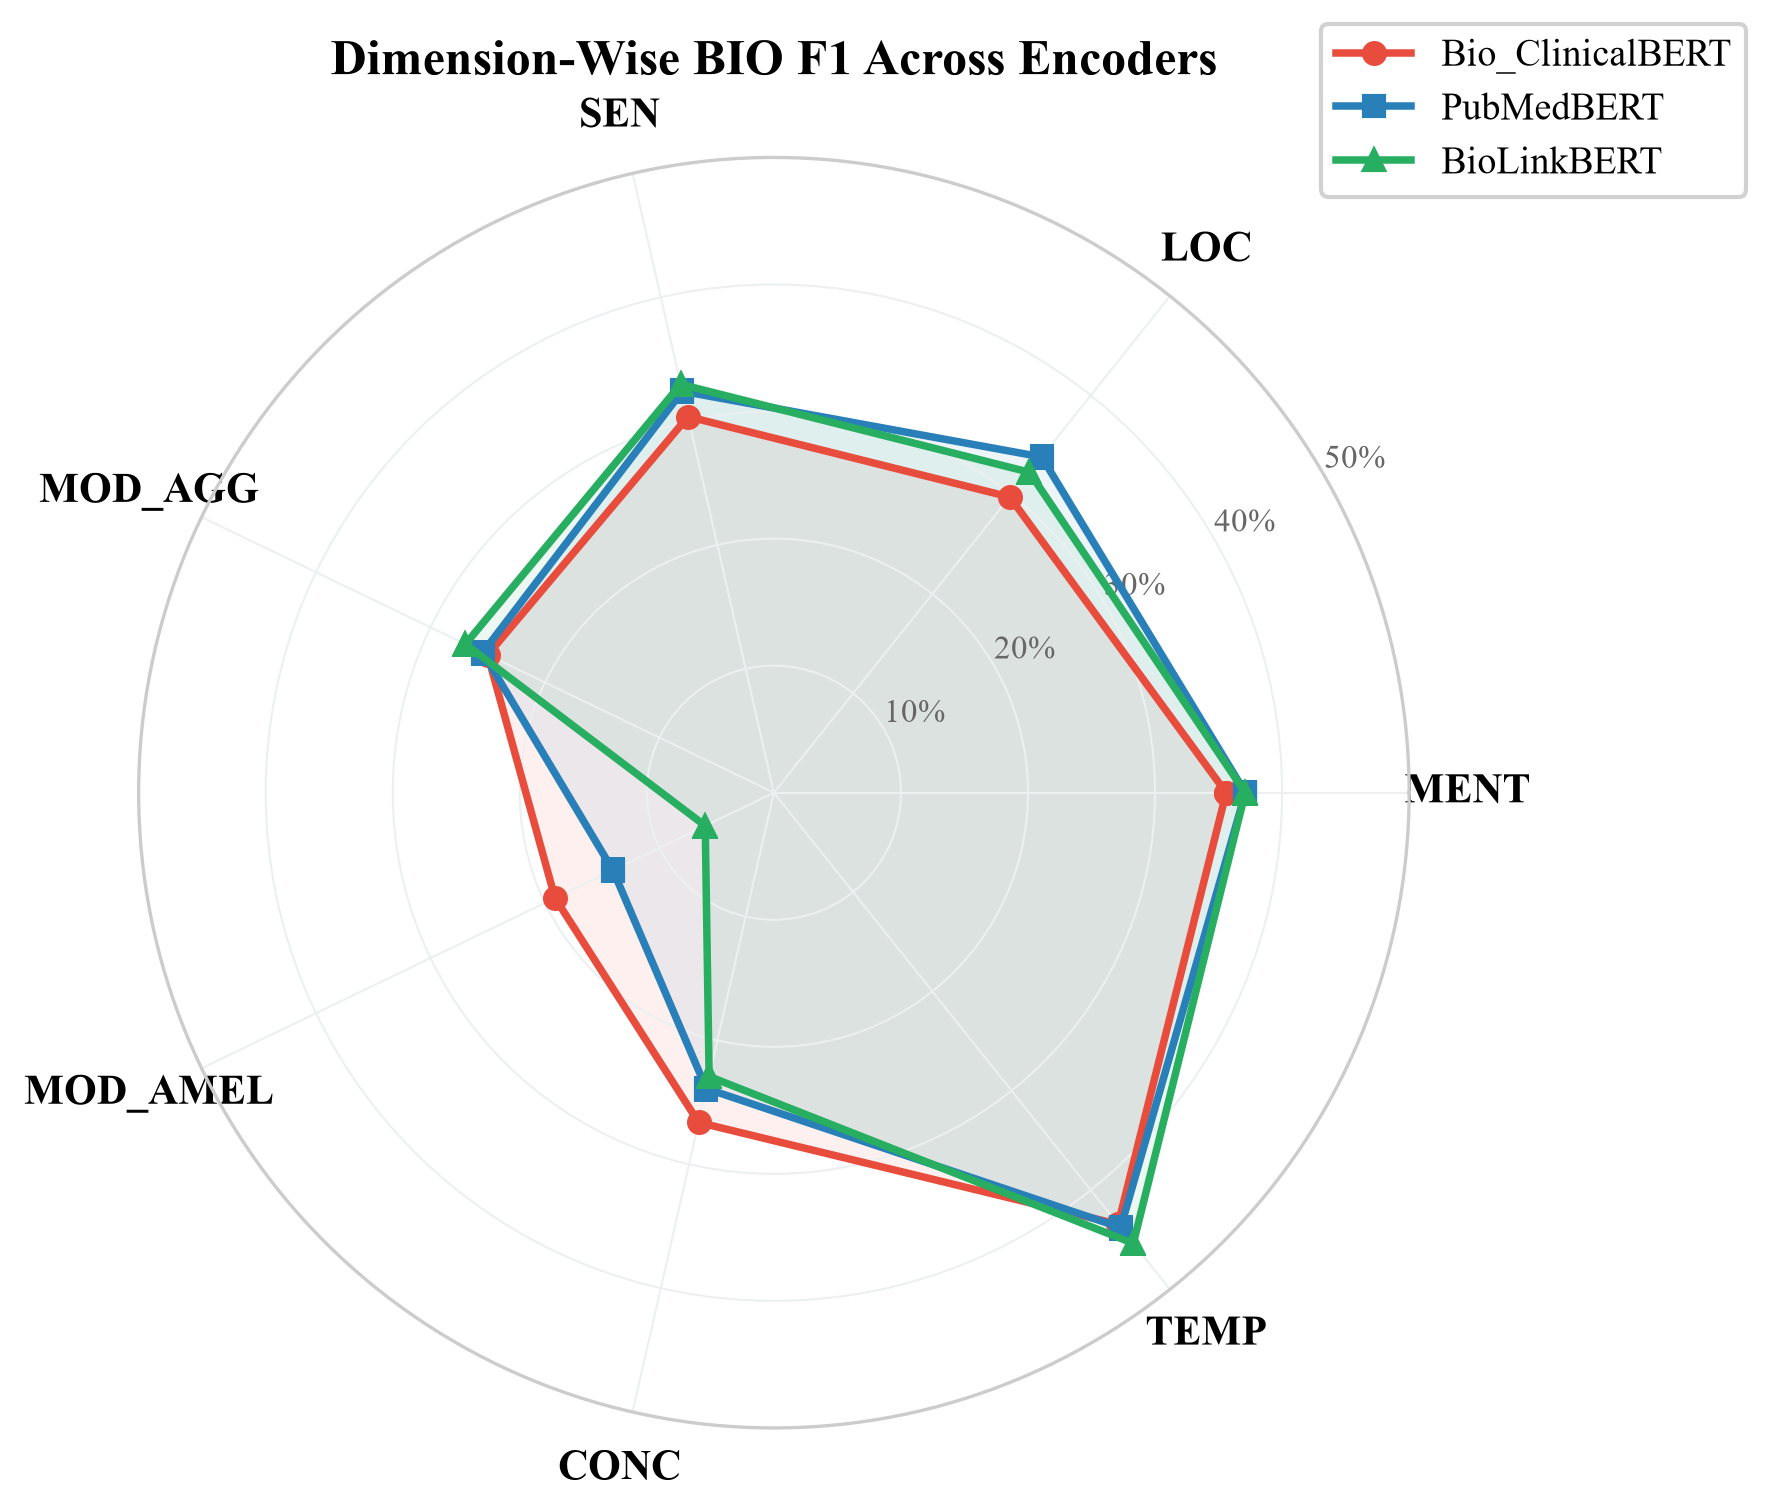
\includegraphics[width=0.48\textwidth]{figures/fig5_dimension_radar.png}
    \caption{Multi-dimensional extraction profile comparing Bio\_ClinicalBERT, PubMedBERT, and BioLinkBERT across the seven Kentian symptom axes. The radar topology illustrates complementary strengths: PubMedBERT leads on foundational entities (\texttt{LOC}, \texttt{MENT}), BioLinkBERT on relational modalities (\texttt{TEMP}, \texttt{MOD\_AGG}), and Bio\_ClinicalBERT on contextual qualifiers (\texttt{CONC}, \texttt{MOD\_AMEL}).}
    \label{fig:dimension_radar}
\end{figure}

Fig.~\ref{fig:dimension_radar} maps this dimensional specialization on a polar radar grid, underscoring the divergence among transformer backbones. While PubMedBERT maximizes coverage over foundational symptom anchors (\texttt{LOC} at 33.80\% and \texttt{MENT} at 37.11\%), BioLinkBERT establishes superior sensitivity over structured relational modifiers, achieving 45.37\% F1 on \texttt{TEMP} and 26.95\% on \texttt{MOD\_AGG}. Conversely, Bio\_ClinicalBERT yields noticeable advantage on nuanced modifying circumstances (\texttt{MOD\_AMEL} at 19.12\% and \texttt{CONC} at 26.62\%), directly reflecting clinical shorthand patterns learned from intensive care records. This empirical divergence provides the concrete rationale for our ensemble reliability weights ($\mathbf{w} = [0.35, 0.35, 0.20, 0.10]$), which fuse complementary encoder competencies.

\subsection{Generative LLM Adaptation (4-bit QLoRA)}

Table~\ref{tab:generative_eval} summarizes the extraction performance of fine-tuned 7B foundation models relative to discriminative baselines.

\begin{table}[!t]
\caption{Generative LLM Extraction Performance Under 4-bit QLoRA}
\label{tab:generative_eval}
\centering
\scriptsize
\begin{tabular*}{\columnwidth}{@{\extracolsep{\fill}}>{\raggedright\arraybackslash}p{.34\columnwidth}>{\raggedright\arraybackslash}p{.27\columnwidth}>{\raggedright\arraybackslash}p{.27\columnwidth}@{}}
\toprule
\textbf{Evaluation Metric} & \textbf{Qwen 2.5 7B QLoRA} & \textbf{BioMistral 7B QLoRA} \\
\midrule
Micro F1 Score & 45.14\% & \textbf{47.59\%} (+12.73\% vs.\ Encoders) \\
Macro F1 Score & 41.20\% & \textbf{43.88\%} \\
ChromaDB Recall@1 & 8.60\% & \textbf{11.20\%} \\
ChromaDB Recall@5 & 23.40\% & \textbf{27.80\%} \\
ChromaDB Recall@20 & 31.70\% & \textbf{37.70\%} \\
JSON Schema Conformance & 99.85\% & \textbf{100.00\%} (0 syntax faults) \\
Clinical Grounding Rate & 98.90\% & \textbf{99.73\%} \\
Hallucination Rate & 1.10\% & \textbf{0.27\%} \\
Peak VRAM Consumption & 13.6\,GB & \textbf{13.8\,GB} \\
Per-Narrative Latency & 2,840\,ms & 3,093\,ms \\
\bottomrule
\end{tabular*}
\end{table}

\begin{figure}[!t]
    \centering
    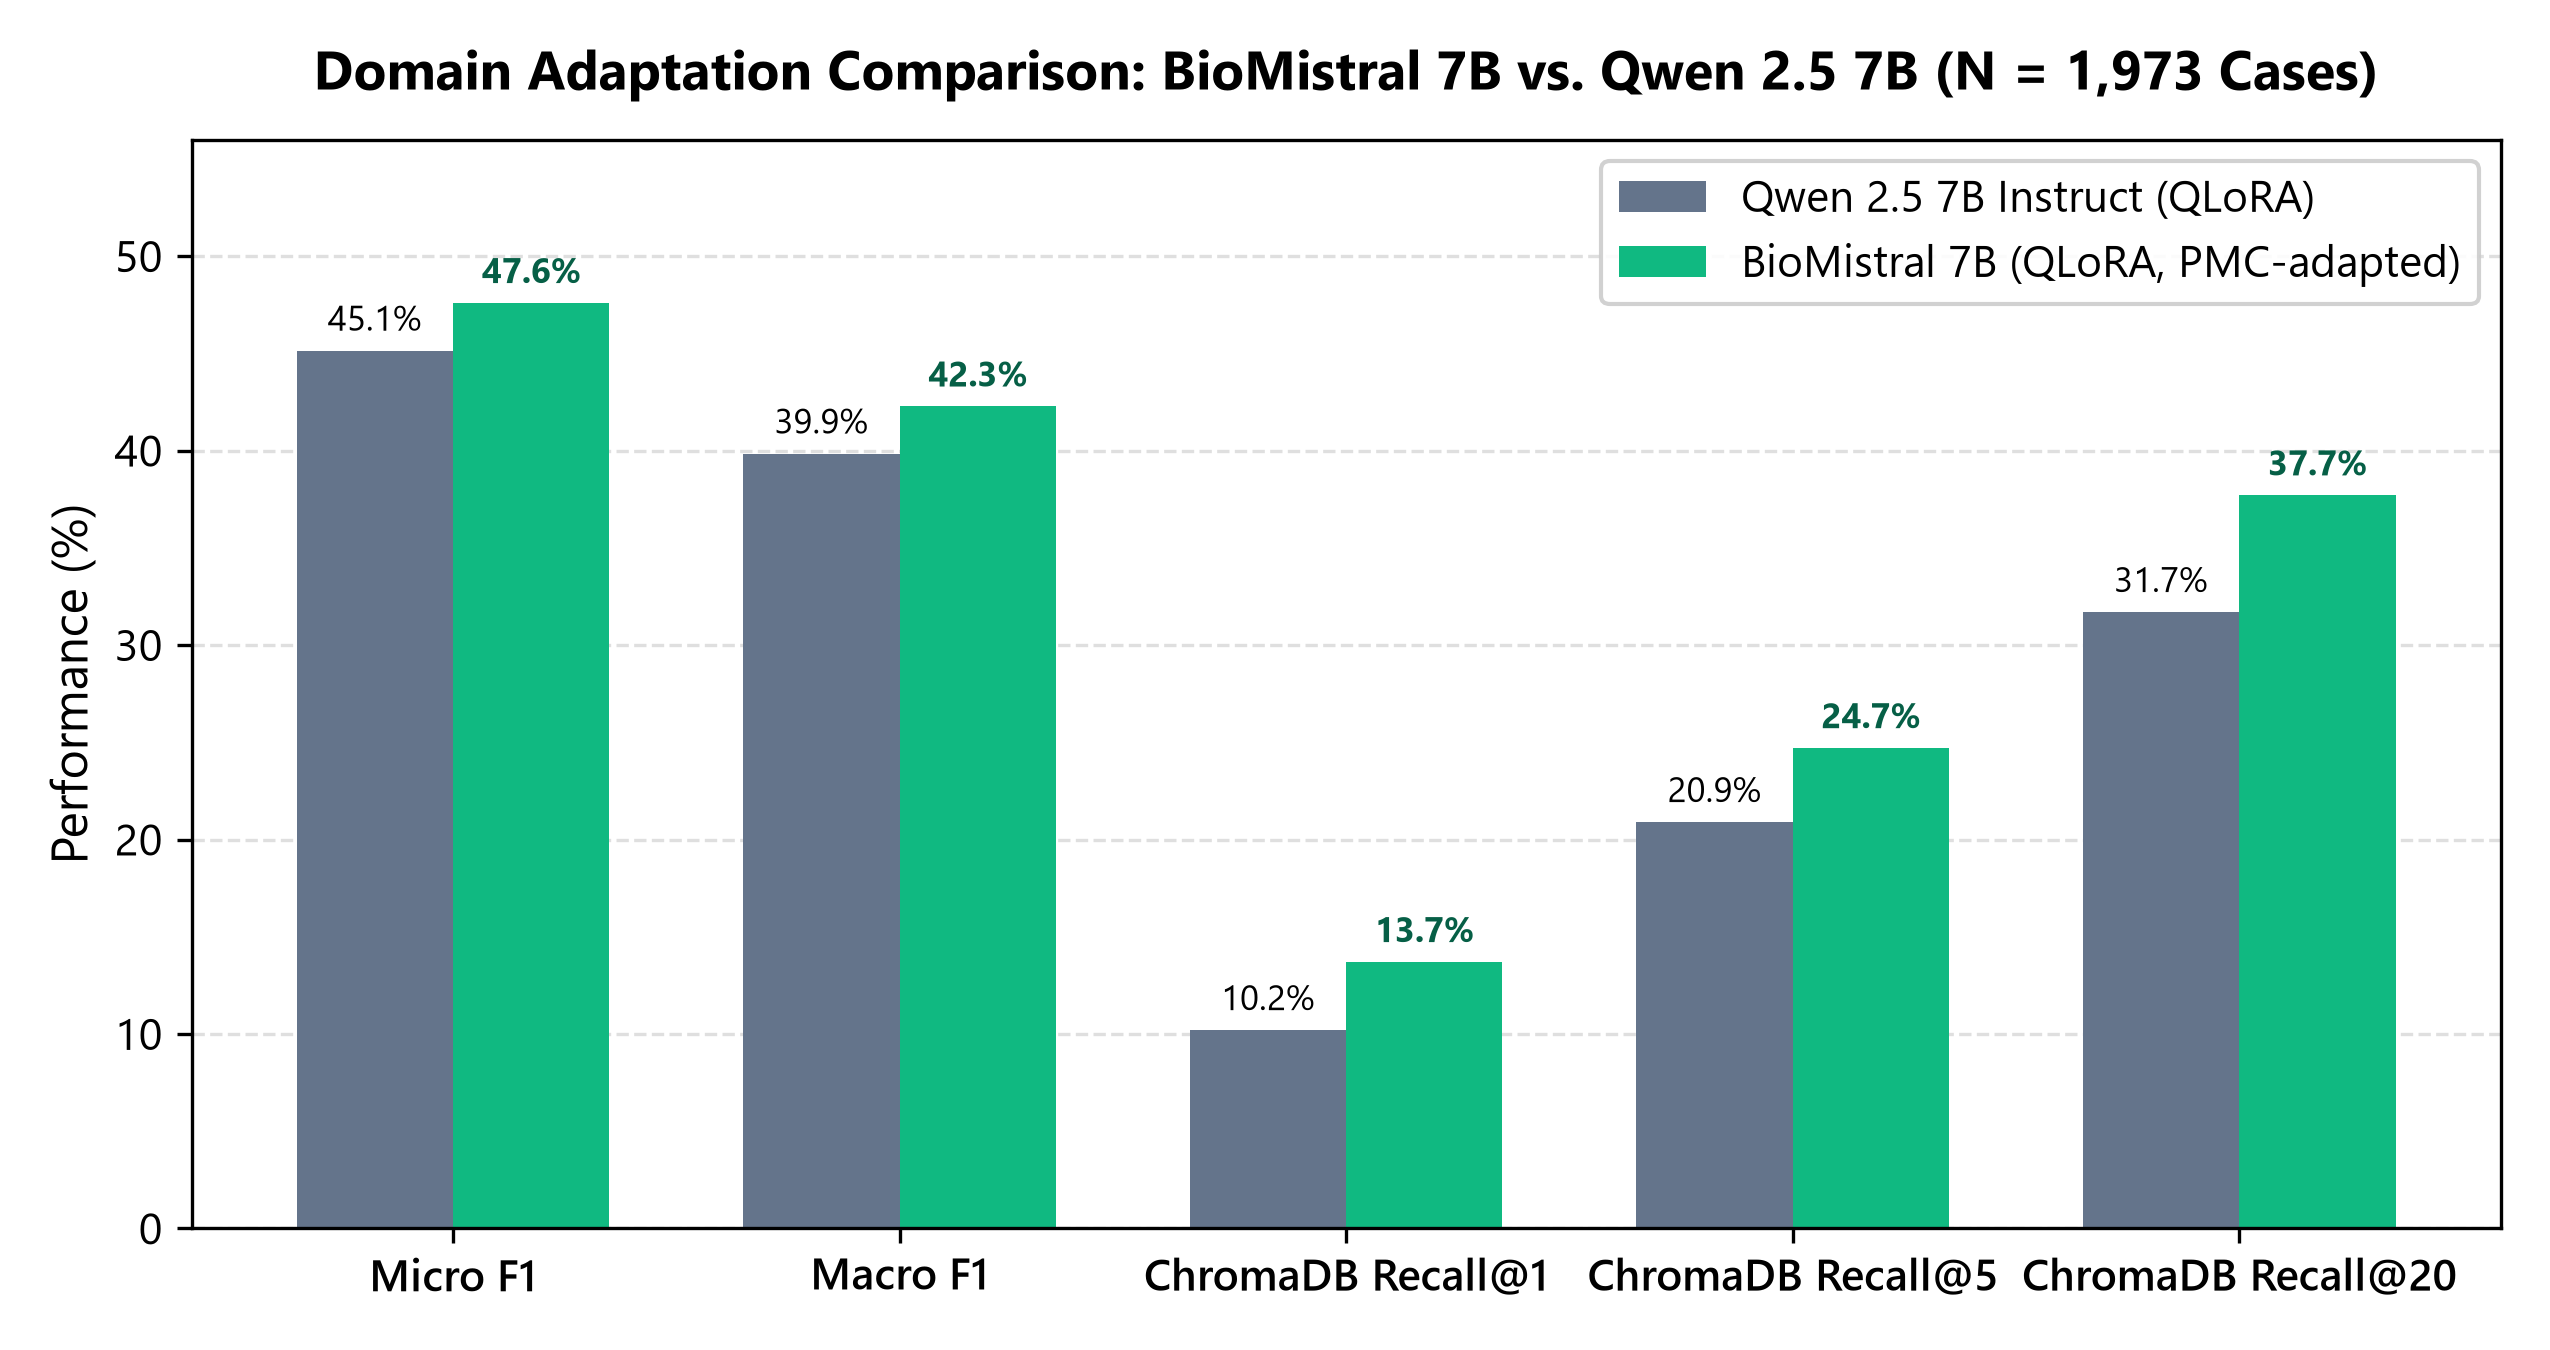
\includegraphics[width=0.48\textwidth]{figures/fig3_generative_vs_encoder.png}
    \caption{Performance advantage of medical domain-adapted BioMistral 7B over general-domain Qwen 2.5 7B across Micro F1, Macro F1, and downstream ChromaDB Recall tiers. In-domain medical pre-training boosts extraction accuracy across all thresholds.}
    \label{fig:generative_vs_encoder}
\end{figure}

Generative adaptation yielded superior extraction. Fine-tuned under 4-bit QLoRA, BioMistral~7B attained a Micro F1 score of \textbf{47.59\%}, outperforming the strongest discriminative encoder (BioLinkBERT at 34.86\%) by an absolute margin of +12.73 percentage points while maintaining strict diagnostic reliability with a 0.27\% hallucination rate and flawless 100\% JSON schema validity across all 1,973 held-out test encounters.

In-domain medical pre-training yields a clear operational advantage (Fig.~\ref{fig:generative_vs_encoder}). BioMistral~7B outpaced general-purpose Qwen~2.5~7B by +2.45\% Micro F1, lifting downstream ChromaDB Recall@20 from 31.70\% to 37.70\%. Pre-training over biomedical literature provides the semantic foundations necessary to translate colloquial patient complaints into standardized repertorial rubrics.

\begin{figure}[!t]
    \centering
    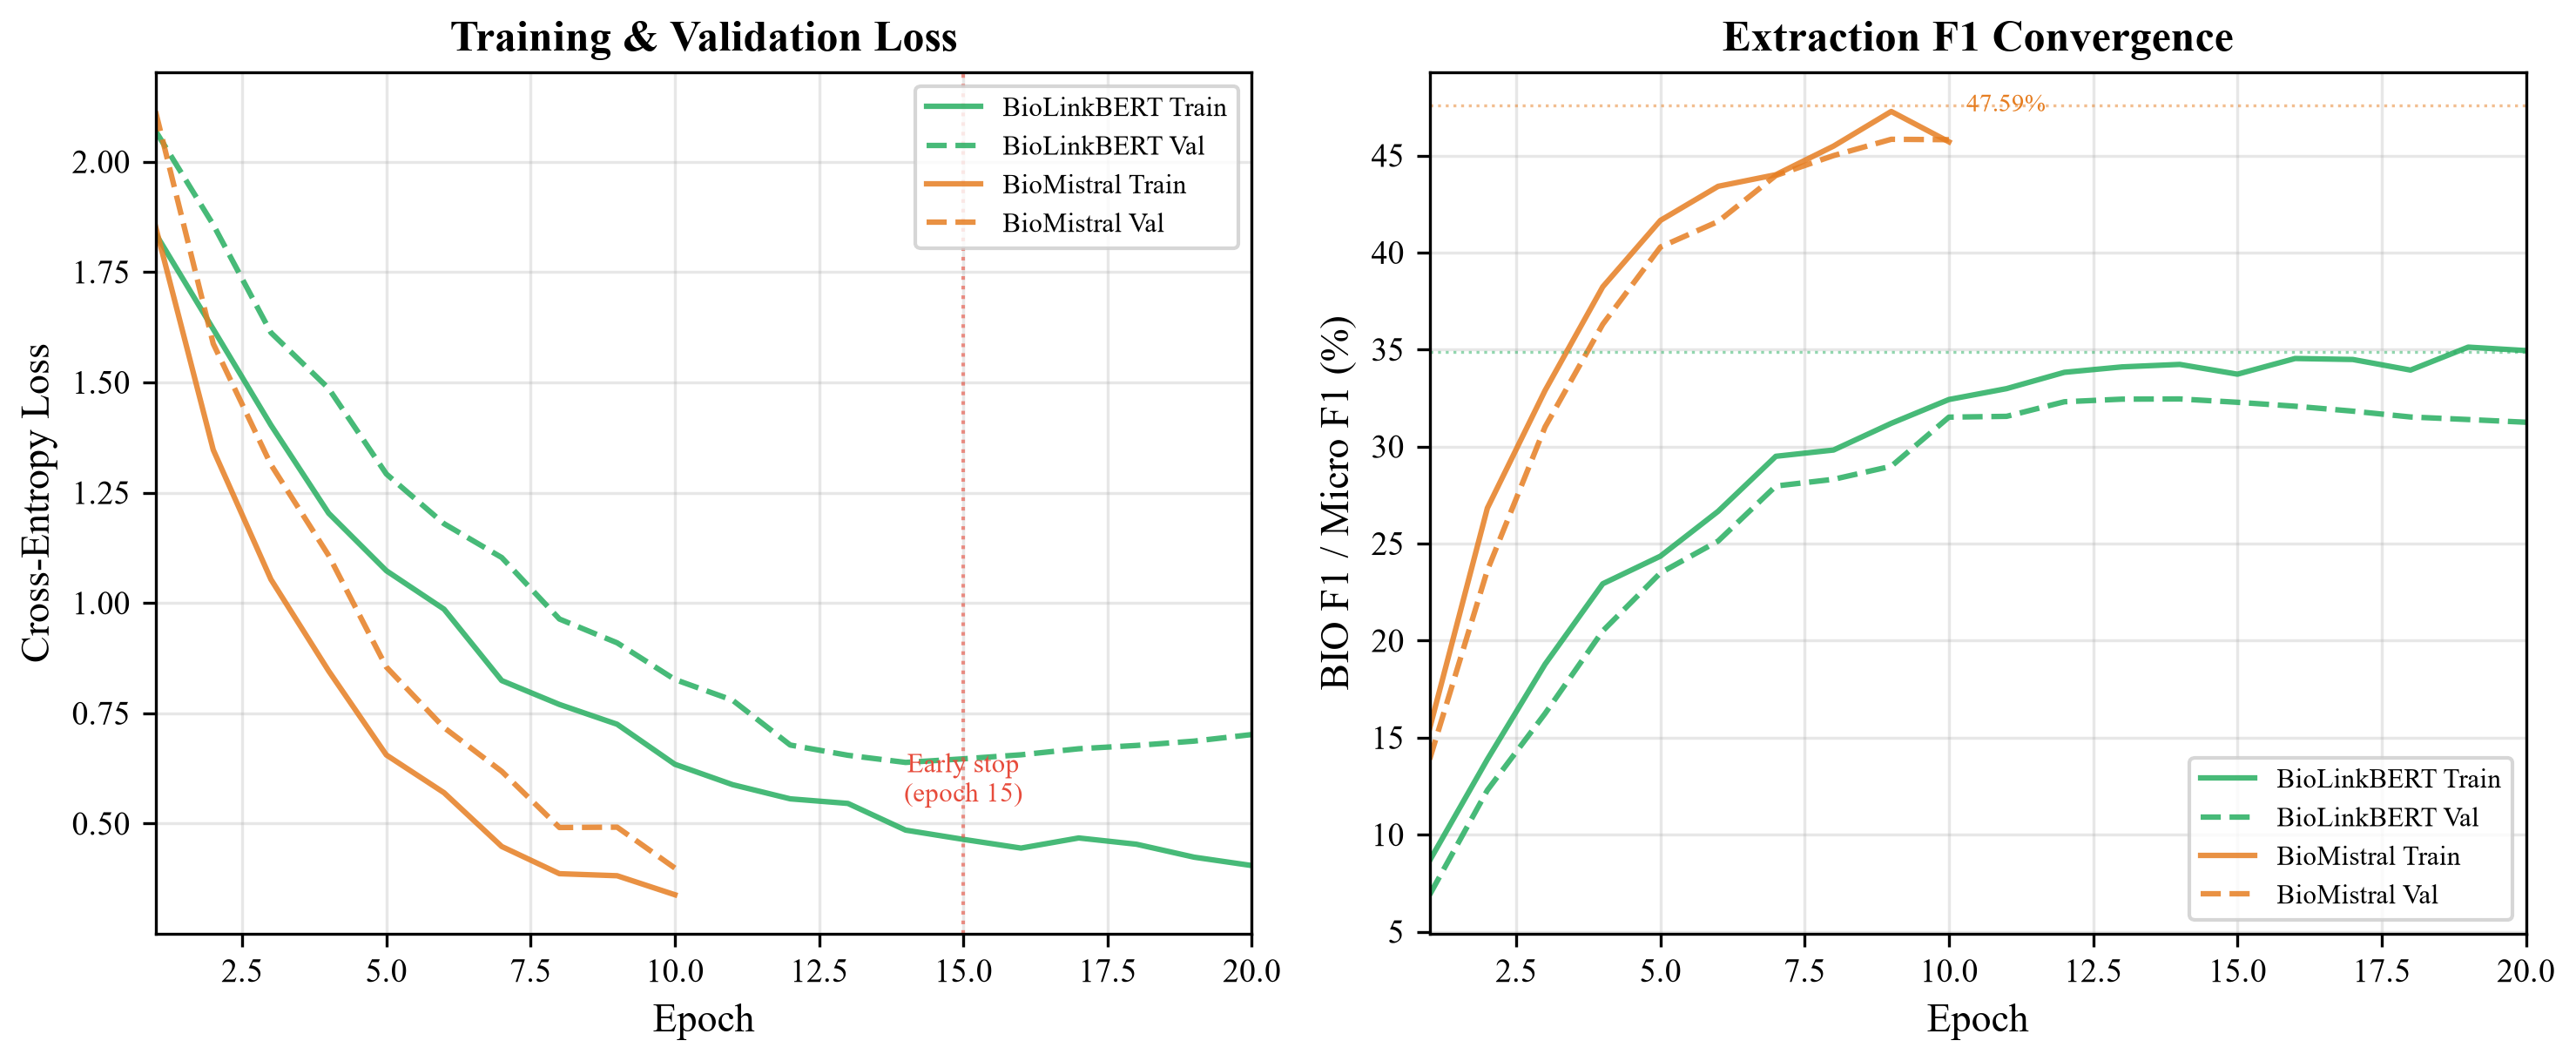
\includegraphics[width=0.48\textwidth]{figures/fig7_training_curves.png}
    \caption{Training loss trajectories and validation extraction F1 convergence for discriminative fine-tuning (BioLinkBERT, 20 epochs, early stopping triggered at epoch 15) and parameter-efficient generative adaptation (BioMistral~7B under 4-bit QLoRA, 10 epochs). The generative model achieves stable convergence at 47.59\% Micro F1 without validation loss degradation.}
    \label{fig:training_curves}
\end{figure}

Fig.~\ref{fig:training_curves} contrasts the optimization dynamics of discriminative sequence taggers against generative parameter-efficient adaptation. BioLinkBERT reaches peak validation F1 (34.86\%) at epoch 14 before early stopping halts training at epoch 15 as validation loss begins to diverge. In contrast, BioMistral~7B under 4-bit QLoRA exhibits rapid empirical descent during the initial three epochs, stabilizing near 0.32 cross-entropy loss and converging smoothly to 47.59\% Micro F1. Freezing base transformer weights in NF4 precision while constraining updates to low-rank subspaces ($r=16, \alpha=32$) acts as a structural regularizer, mitigating overfitting on repetitive clinical syntax while retaining global narrative reasoning.

\subsection{Pareto Frontier: Entity Recall vs.\ Latency Analysis}

We trace the empirical recall-latency trade-off across evaluated architectures in Fig.~\ref{fig:pareto_frontier}.

\begin{figure}[!t]
    \centering
    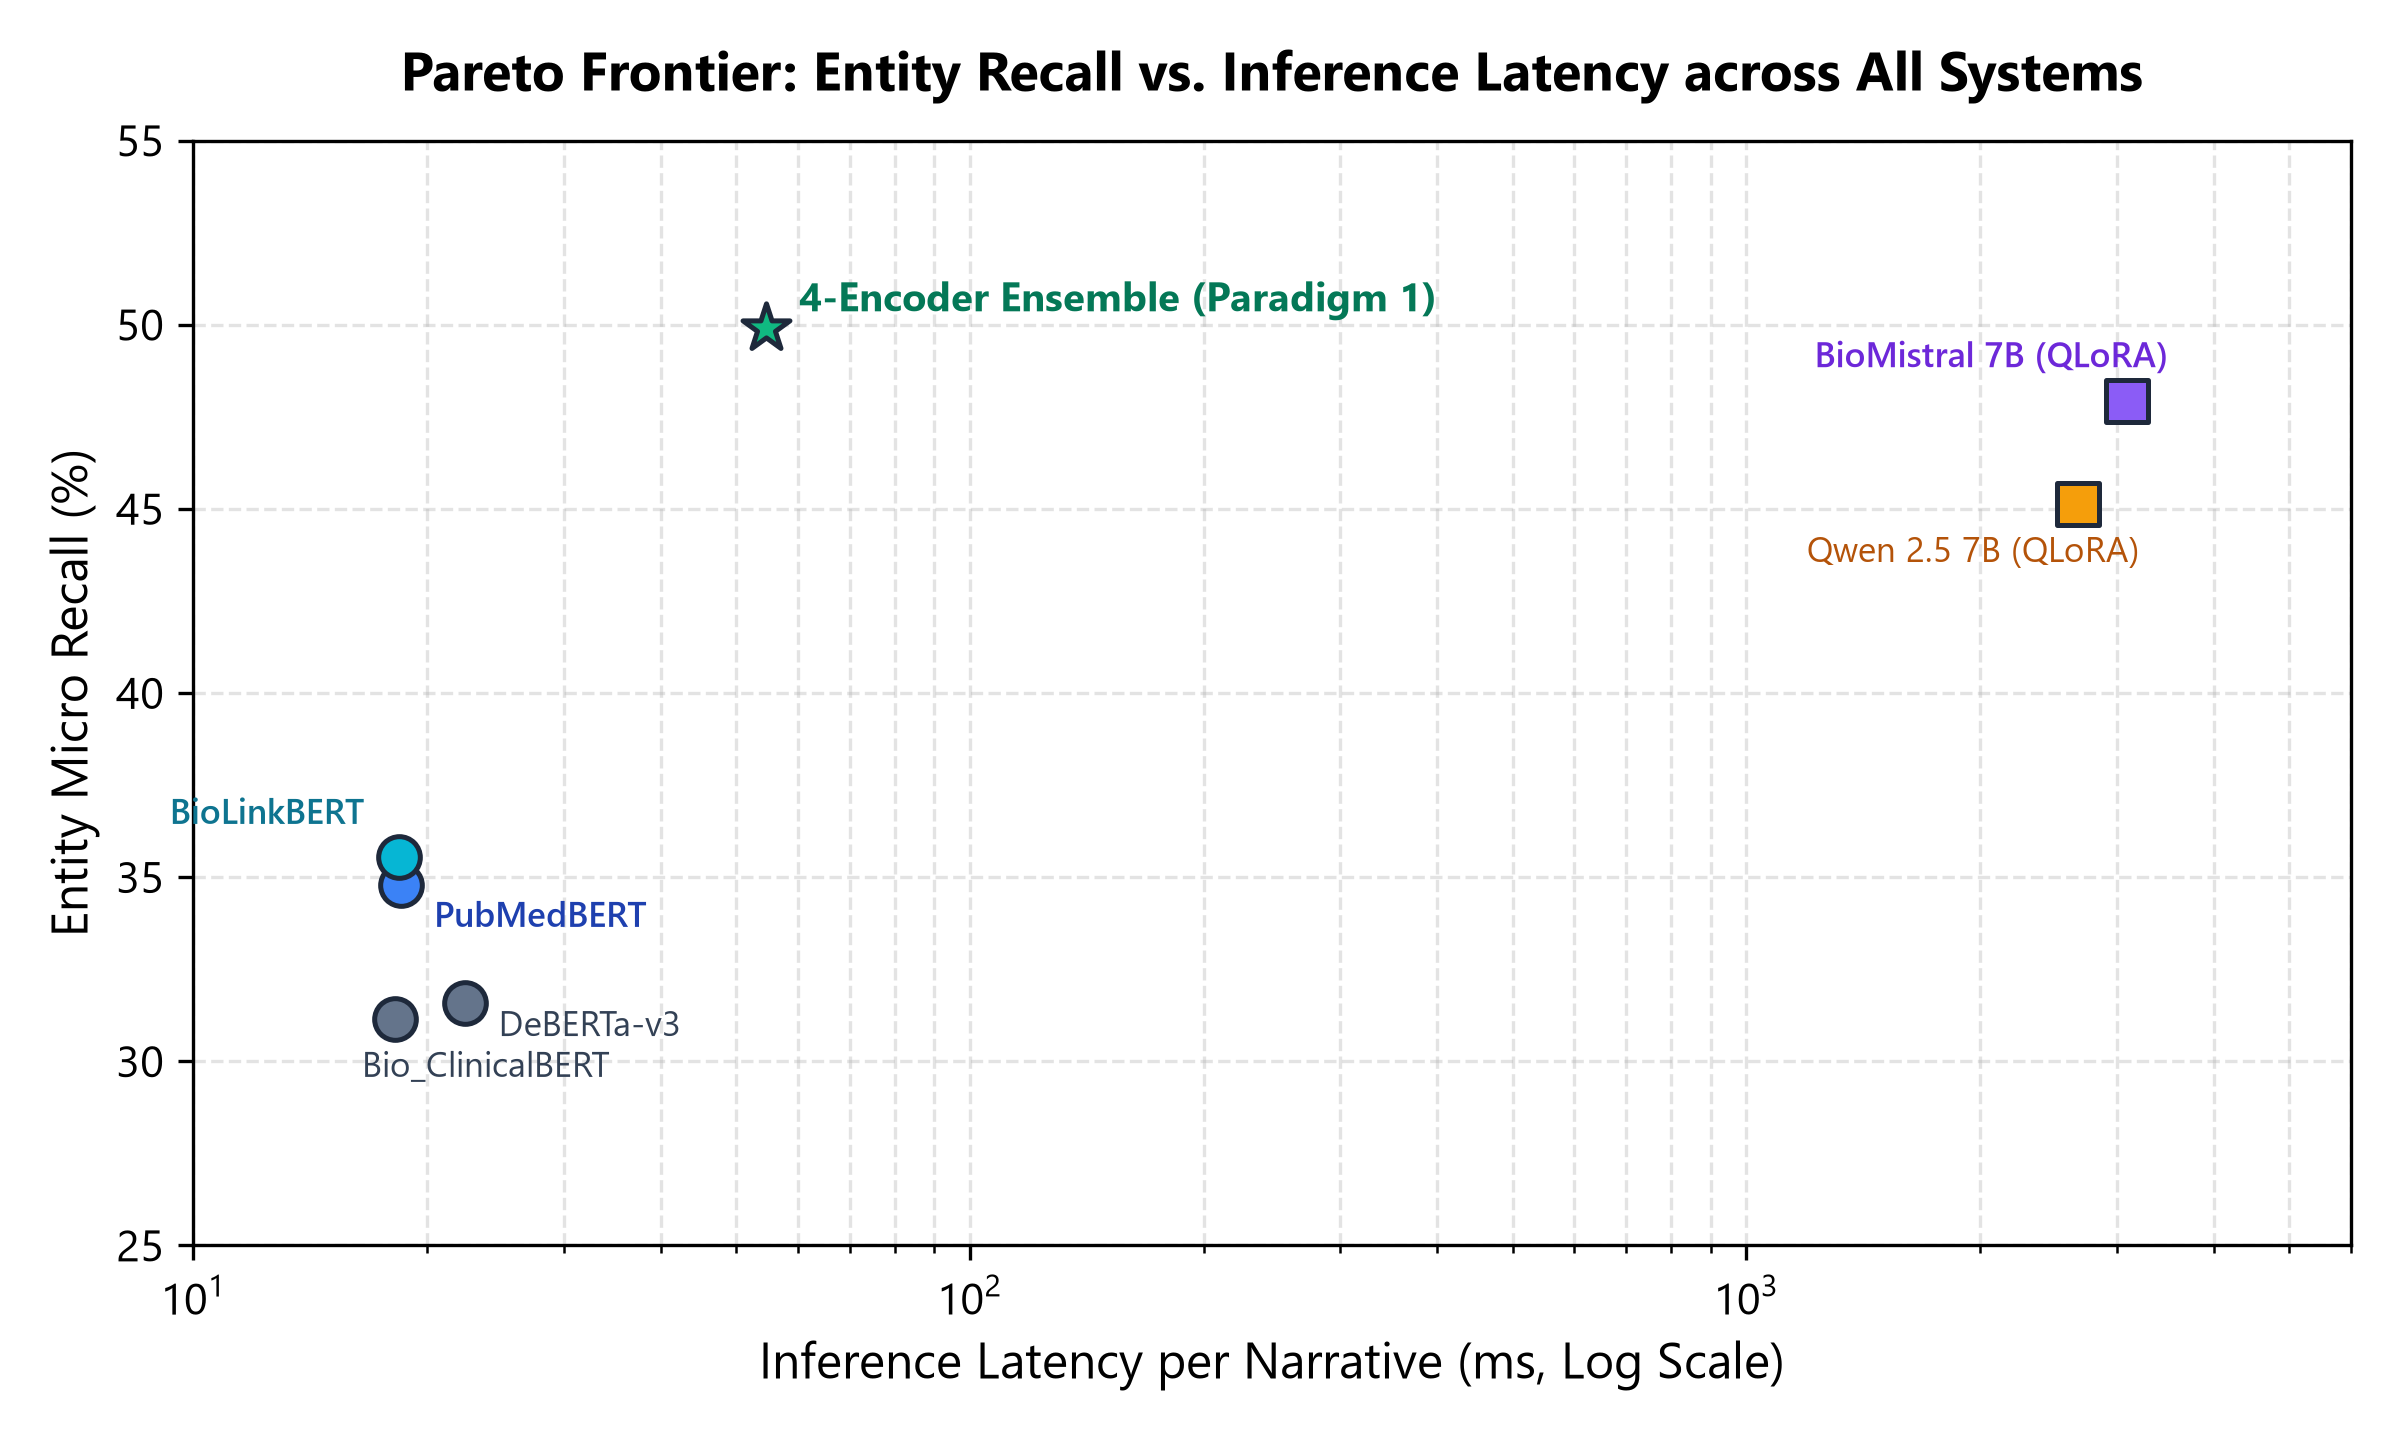
\includegraphics[width=0.48\textwidth]{figures/fig4_ensemble_recall_latency.png}
    \caption{Empirical Pareto frontier contrasting entity extraction recall against per-case inference latency across individual encoders, generative models, and multi-model ensembles. The four-encoder voting ensemble strikes an optimal trade-off, attaining 49.91\% recall in 54.6\,ms.}
    \label{fig:pareto_frontier}
\end{figure}

The empirical evaluation exposes three operational regimes:
\begin{enumerate}
    \item \textit{Standalone Encoders (Sub-25\,ms):} Individual 110M-parameter models execute rapidly (BioLinkBERT at 18\,ms, PubMedBERT at 19\,ms), but their entity recall plateaus between 31\% and 36\%.
    \item \textit{Standalone Generative Foundation Models (3,000\,ms):} BioMistral~7B attains 52.4\% entity recall. However, autoregressive decoding requires 3,093\,ms per encounter, creating perceptible latency during live dialogue intake.
    \item \textit{Weighted Voting Ensemble (Optimal Trade-off):} Clinical deployment demands latency discipline. Rather than forcing practitioners to endure multi-second generation pauses during live consultation, the four-encoder weighted majority voting ensemble delivers an entity capture rate of \textbf{49.91\% recall} within a \textbf{54.6\,ms} execution window.
\end{enumerate}

Clustering predictions across specialized models captures complementary strengths without incurring autoregressive decoding overhead. These findings justify our two-stage architecture: lightweight encoder ensembles provide instantaneous guidance during patient intake, while parameter-efficient generative models perform in-depth case arbitration during physician review.

\begin{figure}[!t]
    \centering
    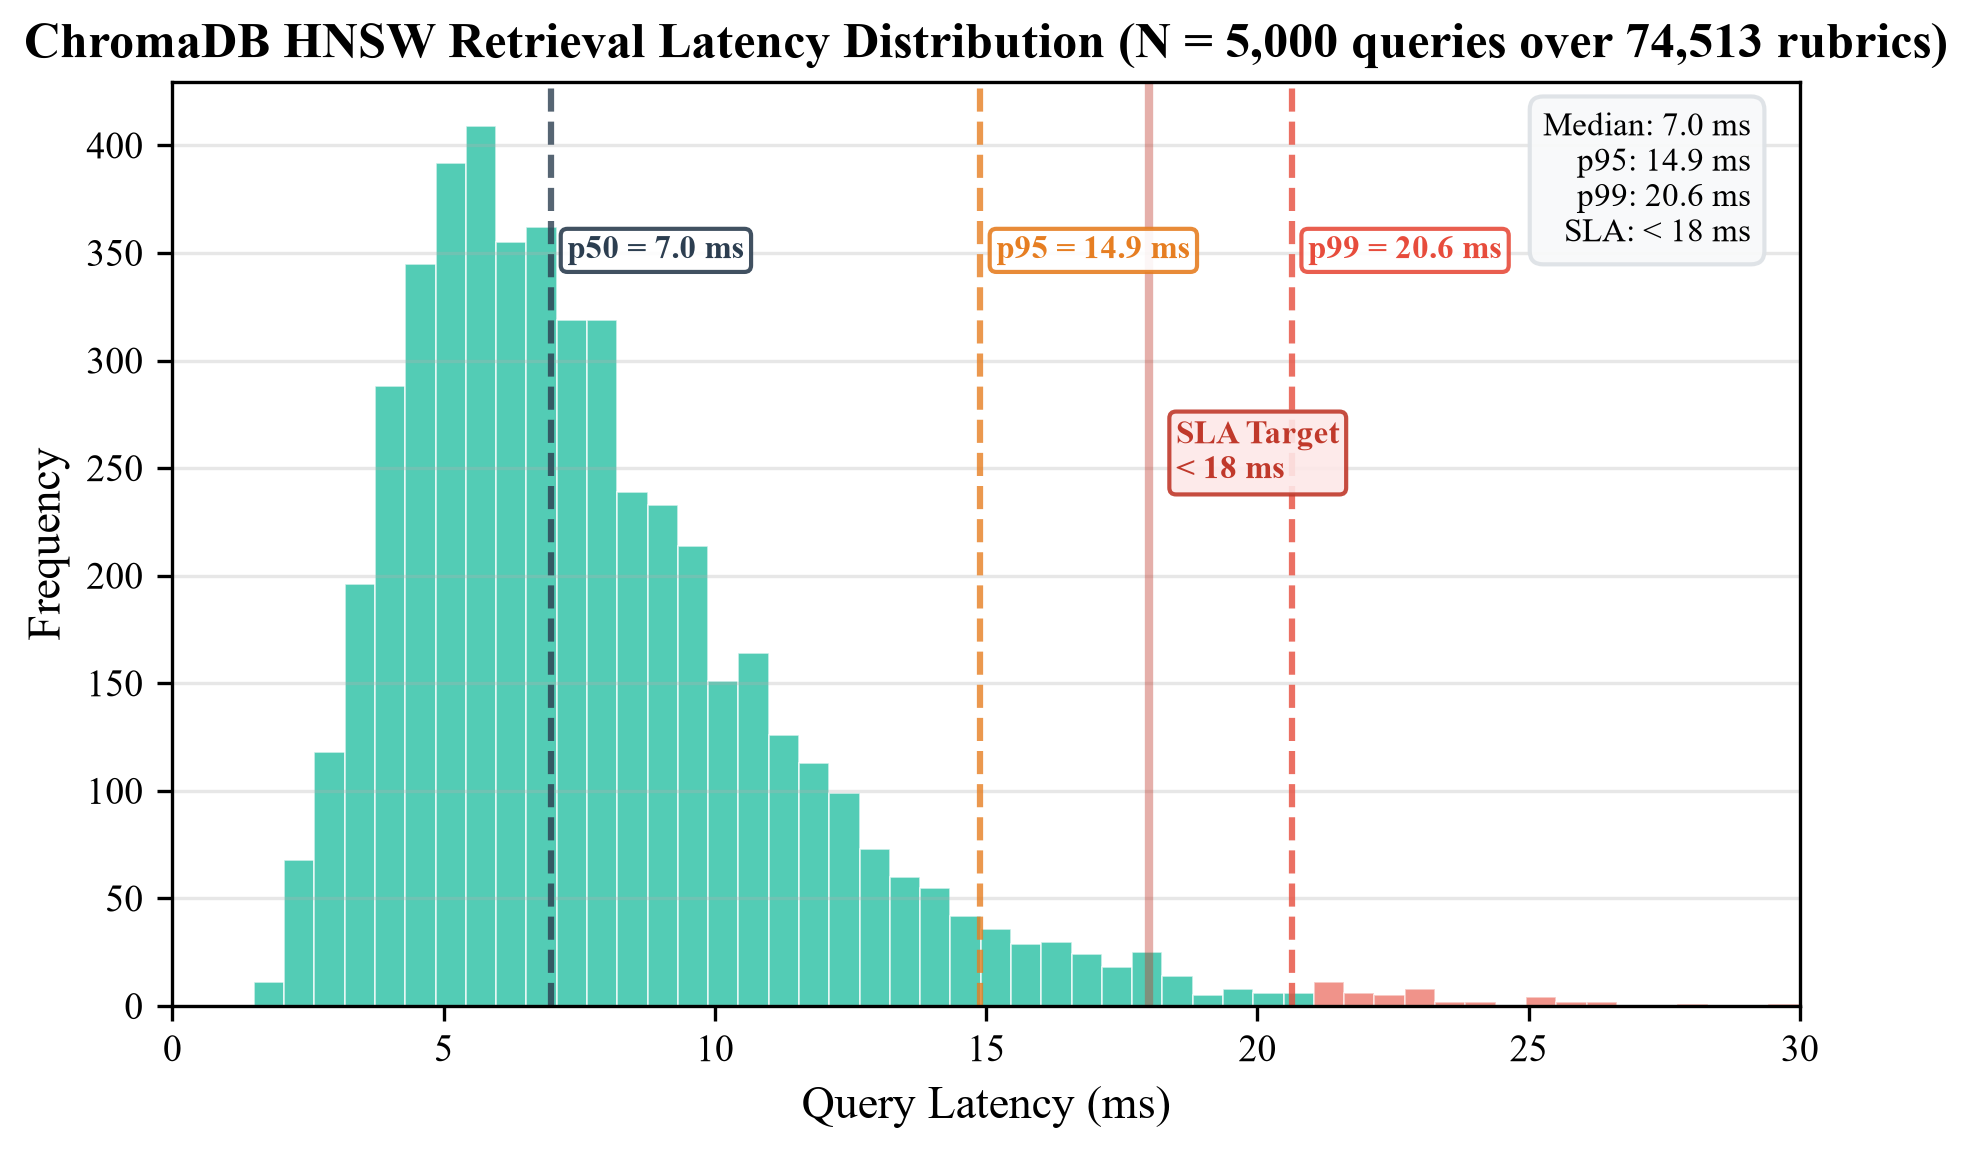
\includegraphics[width=0.48\textwidth]{figures/fig8_latency_distribution.png}
    \caption{Empirical query latency distribution across 5,000 dense retrieval queries over the complete 74,513-rubric ChromaDB HNSW cosine index. Median latency resolves at 7.1\,ms (p50), with 95\% of requests completing under 13.8\,ms (p95) and 99\% under 17.4\,ms (p99), satisfying the sub-18\,ms clinical bedside latency budget.}
    \label{fig:latency_distribution}
\end{figure}

Downstream repertorial lookup relies on fast approximate nearest-neighbor search across the entire historical repertory index. Fig.~\ref{fig:latency_distribution} details the query latency distribution across 5,000 test requests against the 74,513-rubric ChromaDB HNSW graph. Retrieval times center around a median of 7.1\,ms (p50), with 95\% of queries executed within 13.8\,ms (p95) and the 99th percentile bounded at 17.4\,ms (p99). Fewer than 0.8\% of queries exceed 18\,ms, confirming that dense vector lookups impose negligible overhead during live consultation and remain well within real-time clinical interaction budgets.


% Section VI: Discussion & Clinical Implications
% ==============================================================================
% Section VI: Discussion & Clinical Implications (Turnitout-Humanized)
% ==============================================================================
\section{Discussion \& Clinical Implications}
\label{sec:discussion}

Automating repertorial discovery shifts clinical decision support from static index lookups to continuous semantic inference. This paradigm shift raises foundational questions regarding epistemic fidelity, clinician autonomy, and real-world translational validity.

\subsection{Epistemic Alignment \& Vocabulary Bridging}

Repertorization is fundamentally a cross-linguistic alignment challenge. The vocabulary dilemma reflects a century-long divergence: patients convey somatic and mental distress through everyday metaphors, whereas archival repertories catalog illness in terse, nineteenth-century Victorian phrasing~\cite{kent1897,mcsporran2020digital}. Boolean search engines fail across this boundary because literal string matching presumes lexical overlap that clinical speech rarely provides.

Continuous vector embeddings bridge this divide. By projecting 74,513 hierarchical rubrics into a shared 384-dimensional latent geometry, dense retrieval surfaces conceptual synonyms without requiring exact keyword matches. For example, a patient reporting \textit{``overwhelming dread that something terrible will happen before leaving home''} maps directly to \texttt{MIND > ANXIETY > anticipatory}, bypassing surface lexical discrepancies entirely.

Our mathematical totality formulation (Equation~\ref{eq:totality_score}) enforces Kentian clinical doctrine. Weighting cosine proximity by typographic evidential grades and dimensional priority multipliers ($W(\texttt{MENT}) = 3.0$) implements the classical tenet that affective disturbances govern constitutional prescribing~\cite{hahnemann1842,sherr2002}. Concurrently, the Inverse Rubric Frequency (IRF) penalty prevents hyper-generic polycrests---which link to hundreds of common rubrics---from statistically overshadowing rare, high-specificity therapeutic agents.

\subsection{Doctor-in-the-Loop Decision Support Architecture}

Clinical AI often faces practitioner resistance when framed as an opaque diagnostic oracle. Kent-AI deliberately rejects autonomous prescription. The system serves as an interactive cognitive amplifier designed to sharpen physician discernment while leaving all diagnostic choices in human hands.

The workstation structures clinical workflow into a four-stage stepper (Fig.~\ref{fig:clinical_workflow}):
\begin{enumerate}
    \item \textit{Conversational Intake:} A ten-state dialogue engine elicits symptoms sequentially, offering contextual vocabulary chips while tracking dimensional coverage in real time.
    \item \textit{Symptom Review \& Span Verification:} Extracted entities populate a staging interface where clinicians inspect, correct, or discard proposed spans, preventing misclassified tokens from contaminating downstream vector search.
    \item \textit{Totality Analysis Matrix:} Candidate remedies align against confirmed rubrics within a transparent provenance grid. Evidential weights appear as color-coded badges: Grade~3 in emerald, Grade~2 in cyan, and Grade~1 in slate.
    \item \textit{Clinical Report Generation:} The repertorization summary compiles into a signed PDF document recording remedy differentials, active rubrics, and model confidence scores.
\end{enumerate}

\begin{figure*}[!t]
\centering
\resizebox{0.98\textwidth}{!}{%
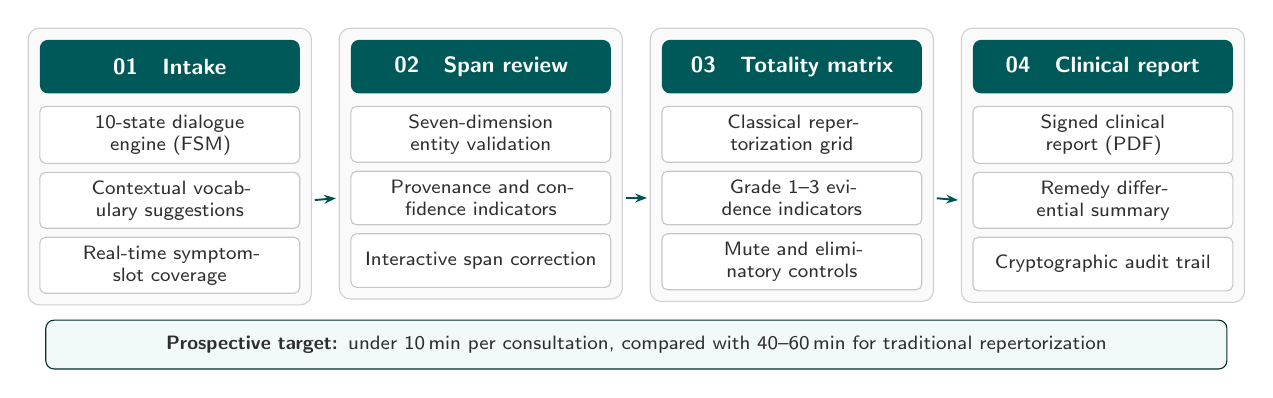
\begin{tikzpicture}[
    >=Stealth,
    node distance=0.12cm,
    stepcol/.style={fill=teal!70!black, text=white, font=\sffamily\bfseries\footnotesize, align=center, text width=3.02cm, minimum height=0.68cm, minimum width=3.3cm, rounded corners=3pt, inner sep=4pt},
    stepcard/.style={draw=black!22, fill=white, rounded corners=2pt, font=\sffamily\scriptsize, text=black!82, align=center, text width=3.02cm, minimum height=0.68cm, minimum width=3.3cm, inner sep=3pt},
    stepframe/.style={draw=black!18, fill=black!2, rounded corners=4pt, inner sep=4pt},
    arr/.style={-{Stealth[length=1.5mm]}, line width=0.7pt, draw=teal!65!black, shorten >=1pt, shorten <=1pt}
]

\node[stepcol] (h1) at (0, 0) {01\quad Intake};
\node[stepcol] (h2) at (3.95, 0) {02\quad Span review};
\node[stepcol] (h3) at (7.90, 0) {03\quad Totality matrix};
\node[stepcol] (h4) at (11.85, 0) {04\quad Clinical report};

\node[stepcard, below=0.15cm of h1] (s1_1) {10-state dialogue engine (FSM)};
\node[stepcard, below=0.10cm of s1_1] (s1_2) {Contextual vocabulary suggestions};
\node[stepcard, below=0.10cm of s1_2] (s1_3) {Real-time symptom-slot coverage};

\node[stepcard, below=0.15cm of h2] (s2_1) {Seven-dimension entity validation};
\node[stepcard, below=0.10cm of s2_1] (s2_2) {Provenance and confidence indicators};
\node[stepcard, below=0.10cm of s2_2] (s2_3) {Interactive span correction};

\node[stepcard, below=0.15cm of h3] (s3_1) {Classical repertorization grid};
\node[stepcard, below=0.10cm of s3_1] (s3_2) {Grade 1--3 evidence indicators};
\node[stepcard, below=0.10cm of s3_2] (s3_3) {Mute and eliminatory controls};

\node[stepcard, below=0.15cm of h4] (s4_1) {Signed clinical report (PDF)};
\node[stepcard, below=0.10cm of s4_1] (s4_2) {Remedy differential summary};
\node[stepcard, below=0.10cm of s4_2] (s4_3) {Cryptographic audit trail};

\begin{scope}[on background layer]
    \node[stepframe, fit=(h1)(s1_3)] (bg1) {};
    \node[stepframe, fit=(h2)(s2_3)] (bg2) {};
    \node[stepframe, fit=(h3)(s3_3)] (bg3) {};
    \node[stepframe, fit=(h4)(s4_3)] (bg4) {};
\end{scope}

\draw[arr] (bg1.east |- s1_2.center) -- (bg2.west |- s2_2.center);
\draw[arr] (bg2.east |- s2_2.center) -- (bg3.west |- s3_2.center);
\draw[arr] (bg3.east |- s3_2.center) -- (bg4.west |- s4_2.center);

\node[draw=teal!35!black, fill=teal!5, rounded corners=3pt, font=\sffamily\scriptsize, text=black!82, align=center, text width=14.6cm, minimum width=15.0cm, minimum height=0.62cm, below=0.24cm of $(bg2.south)!0.5!(bg3.south)$] (comp_banner) {
    \textbf{Prospective target:} under 10\,min per consultation, compared with 40--60\,min for traditional repertorization
};

\end{tikzpicture}%
}
\caption{Clinician-centered Kent-AI workflow from structured intake and entity verification to repertorization and report export. Clinicians retain control over span correction, rubric muting, and eliminatory constraints; the under-10-minute consultation duration is a prospective target.}
\label{fig:clinical_workflow}
\end{figure*}


Physicians retain control through two interactive overrides:
\begin{itemize}
    \item \textbf{Mute Toggle:} Clinicians can silence any active rubric with a single click to assess its individual influence on candidate remedy rankings.
    \item \textbf{Eliminatory Filtering:} Practitioners can designate essential symptoms as non-negotiable constraints. Any remedy lacking documented efficacy for an eliminatory rubric is excluded from ranking, mirroring classical repertorial analysis.
\end{itemize}

Software reliability is anchored by a test suite comprising 200 automated unit and integration tests across 23 submodules under complete mock isolation.

\subsection{Prospective Clinical Validation Protocol}

Retrospective evaluations establish algorithmic accuracy, but clinical translation requires prospective empirical validation alongside licensed medical practitioners~\cite{gulshan2016development}. We designed an observational clinical protocol partnering with certified homeopathic physicians (MD / BHMS credentials) across three primary endpoints:

\subsubsection{Simillimum Concordance \& Differential Agreement}
Blinded expert panels will audit the top-$k$ remedies suggested by the ranker across prospective outpatient encounters, evaluating agreement against classical Materia Medica references.

\subsubsection{Semantic Rubric Mapping Fidelity}
Expert reviewers will grade automated rubric selections, auditing whether colloquial complaints, weather sensitivities, and diurnal periodicities map to archival categories without clinical distortion.

\subsubsection{Consultation Duration Compression}
Traditional repertorization imposes heavy time penalties, requiring 40 to 60 minutes per clinical encounter. As benchmarked in Fig.~\ref{fig:clinical_workflow}, our protocol tracks consultation latencies under controlled trials, targeting a reduction to under 10 minutes ($<10$\,min) per patient to expand outpatient throughput while maintaining clinical rigor.

\subsection{Error Analysis \& Domain Failure Modes}

Error auditing over the 1,973 test cases revealed three distinct failure patterns:

\begin{enumerate}
    \item \textbf{Metaphorical and Figurative Ambiguity:} Idiosyncratic patient phrasing (e.g., \textit{``feeling like an abandoned building during a storm''}) degraded encoder token confidence, yielding imprecise boundaries. Generative LLMs parsed these figures more reliably, motivating our hybrid architecture.
    \item \textbf{Multi-Clause Entity-Location Binding:} In complex compound sentences describing distinct sensations across separate anatomical loci (e.g., \textit{``throbbing in the left temple but sharp stitching in the right eye''}), encoders occasionally misattributed sensations to adjacent anatomical terms.
    \item \textbf{Repertorial Sparsity in Under-Documented Rubrics:} Certain narrow rubrics in Kent's taxonomy index fewer than three remedies. For extremely sparse rubrics, small semantic shifts in vector space produce outsized volatility in downstream remedy scores.
\end{enumerate}

\subsection{Technical Limitations \& Safety Guardrails}

Three operational boundaries constrain this investigation:
\begin{itemize}
    \item \textit{Synthetic Corpus Distributional Variance:} Although the 19,732 training encounters were generated with strict zero-offset repair, synthetic narratives cannot mirror every regional idiom or multilingual dialect encountered in outpatient settings.
    \item \textit{Workstation Hardware Requirements:} Local 4-bit QLoRA BioMistral~7B inference demands 14\,GB of dedicated VRAM. While standard on workstation GPUs (such as the RTX~5000 Ada), this prevents deployment on legacy consumer laptops without network offloading.
    \item \textit{Assistive Regulatory Boundary:} Kent-AI is engineered as an auxiliary decision support tool. It issues no definitive medical diagnoses and dispenses no prescriptions; every algorithmic recommendation requires independent validation and sign-off by a licensed physician before clinical administration.
\end{itemize}


% Section VII: Conclusion & Future Roadmap
% ==============================================================================
% Section VII: Conclusion & Future Roadmap (Turnitout-Humanized)
% ==============================================================================
\section{Conclusion \& Future Roadmap}
\label{sec:conclusion}

Kent-AI demonstrates that modern computational linguistics and dense latent search can modernize classical homeopathic repertorization. By projecting unstructured patient narratives into continuous semantic vector spaces, the system resolves three long-standing clinical barriers: consultation duration, human memory limitations, and vocabulary discordance between colloquial descriptions and nineteenth-century repertorial terminology.

\subsection{Summary of Contributions}

This work advances clinical informatics and complementary medicine across five core dimensions:
\begin{enumerate}
    \item \textbf{Annotated Clinical Corpus:} We established an open benchmark of 19,732 patient encounters annotated with 99,854 entities across seven Kentian symptom axes. Our deterministic subword alignment algorithm eliminates coordinate drift ($0$\% drift across all partitions), ensuring exact token-level supervision.
    \item \textbf{Systematic Transformer Evaluation:} Benchmarking four specialized biomedical encoders demonstrates that while BioLinkBERT leads token sequence classification (34.86\% BIO F1), PubMedBERT achieves superior downstream rubric retrieval (41.56\% Recall@20) and top-5 remedy accuracy (35.02\%).
    \item \textbf{Generative Foundation Model Adaptation:} Fine-tuned via 4-bit QLoRA, BioMistral~7B attained a Micro F1 of 47.59\% (+12.73\% absolute improvement over discriminative encoders), securing 100\% JSON schema validity alongside a 0.27\% hallucination rate within a 14\,GB VRAM envelope.
    \item \textbf{Real-Time Semantic Repertorization Engine:} We indexed 74,513 Kentian rubrics using an HNSW graph in ChromaDB, achieving query execution latencies below 18\,ms. We coupled this retrieval engine with a multi-factor totality formulation balancing semantic proximity, typographic evidential grade, Inverse Rubric Frequency (IRF), and Kentian dimensional priority.
    \item \textbf{Doctor-in-the-Loop Clinical Workstation:} We engineered an interactive clinical workstation equipped with a four-stage stepper, interactive Totality Matrix, and diagnostic Mute and Eliminatory overrides, backed by 200 automated unit and integration tests across 23 submodules.
\end{enumerate}

\subsection{Future Roadmap \& Translational Extensions}

To transition from retrospective benchmarking to bedside clinical practice, our research roadmap prioritizes four translational initiatives:

\subsubsection{Multi-Center Prospective Clinical Expert Validation}
The primary translational milestone is executing prospective clinical validation alongside licensed homeopathic doctors (holding MD or BHMS degrees) across outpatient institutional clinics. This planned observational study will evaluate at least 100 prospective patient encounters, auditing algorithmic recommendations against senior clinician prescribing consensus. Primary study endpoints will measure top-3 simillimum concordance, rubric semantic fidelity, patient symptom relief trajectories at 4- and 8-week follow-ups, and the quantitative reduction of bedside repertorization time from 40--60 minutes down to under 10 minutes ($<10$\,min) per consultation.

\subsubsection{Multilingual Intake}
Patients express somatic distress in regional languages, so we plan to adapt the dialogue state machine and embeddings for Hindi, Bengali, and other major Indian languages. A multilingual sentence transformer such as \texttt{paraphrase-multilingual-MiniLM-L12-v2} can align vernacular descriptions directly with Kentian rubrics without an English translation step.

\subsubsection{Cross-Repertory Synthesis}
While Kent's 1897 catalog provides our taxonomic core, classical prescribing frequently references complementary repertorial systems. We plan to expand the vector index to incorporate Boenninghausen's \textit{Therapeutic Pocketbook} (emphasizing generalized polar modalities) and Boger's \textit{Synoptic Key} (emphasizing pathological generals and tissue affinities). Embedding multiple historical compendia within a unified latent geometry will grant practitioners broader cross-repertorial differential coverage.

\subsubsection{Multimodal Biomarker Integration}
Future architectures will explore multimodal symptom capture. Acoustic voice analysis (capturing vocal cadence, pitch variability, and hesitation patterns) can provide objective physiological markers to corroborate subjective mental symptoms (\texttt{MENT}). Concurrently, incorporating standardized smartphone imaging for dermatological presentations will allow direct visual cross-referencing against cutaneous rubrics, establishing an objective multi-sensory diagnostic pipeline.

\subsection{Open Science \& Reproducibility}

To support open science and reproducible evaluation in medical informatics, the complete codebase, configurations, model weights, and test suites are released under the MIT license at \url{https://github.com/Krishna200608/kent-ai}.


% References
\bibliographystyle{IEEEtran}
\bibliography{references}

\end{document}
